% -*-LaTeX-*-

% The log below is the old log from when RCS was being used in
% conjunction with this.
%
% $Log: physical-signals.tex,v $
% Revision 1.11 2010/5/1 Larson
% Revised wording and figures throughout
%
% Revision 1.10  2007/12/25 18:48:47  stiber
% Corrected error in figure caption.
%
% Revision 1.9  2007/12/25 18:08:22  stiber
% Fixed typo.
%
% Revision 1.8  2007/12/25 17:47:45  stiber
% Some final cosmetic changes.
%
% Revision 1.7  2007/12/01 00:35:49  stiber
% Relatively small revisions from notes from Spring 2007. Ready for more
% extensive rewriting.
%
% Revision 1.6  2007/04/10 19:55:29  stiber
% Minor fixes.
%
% Revision 1.5  2007/03/20 23:51:32  stiber
% Cleaned up LaTeX and minor problems.
%
% Revision 1.4  2007/03/04 20:01:34  stiber
% OK, this time I've taken out all references to material in the old
% textbook, adding in additional figures where necessary.
%
% Revision 1.3  2007/03/04 19:33:24  stiber
% Initial revision for stand-alone textbook.
%
% Revision 1.2  2004/03/29 19:55:18  stiber
% Updated for Spring 2004 and new textbook (DSP First).
%
% Revision 1.1  2004/02/19 00:22:15  stiber
% Initial revision
%

\chapter{Signals in the Physical World}
\label{ch:physical-signals}

This chapter introduces the fundamental concepts of multimedia from an
``outside the computer'' perspective. We define the term
``multimedia,'' discuss why it is an important issue, how multimedia
signals (sound, images) are generated in the ``real world'' (by both
natural and artificial means) and how we perceive them. We also
introduce a set of convenient mathematical tools for describing
signals. When you are done with this chapter, we hope you will
appreciate the complexity and importance of multimedia communications
and will be eager to see how signals can be processed by computer.

\section{Multimedia and Sensation}

\begin{quote}
``What can give us surer knowledge than our senses? With what else can
  we better distinguish the true from the false?'' \textit{Lucretius}
\end{quote}

Humans, like any other organisms, depend on their senses to provide
information critical to their development and survival. Over time,
life has evolved sophisticated systems for capturing information about
the physical world. The first senses were almost certainly chemical
--- what we would call taste or smell. These senses have a number of
drawbacks: they typically require close physical presence or even
direct contact, they have poor temporal resolution (you can tell that
someone was cooking onions, but not \emph{when}), and they have poor
spatial resolution (from where is that bad smell coming?). Other
senses --- hearing, seeing, electrical senses that fish have, magnetic
senses that birds have --- allow us to gather information remotely
from the information source.

Given all this, it is perhaps not surprising that people find computer
systems difficult to use, uninspiring, or even objects of
distaste. Computers by and large produce a very impoverished set of
stimuli, composed almost entirely of patterns of light that we must
interpret as text (when people use devices that provide a richer
experience, such as tablets or smartphones, they often mentally
categorize them just that way: as \emph{devices}, not
\emph{computers}). It is only fairly recently that computers have done
much more than this, as processing power and hardware speed has
enabled \emph{multi}media capabilities (though these are almost always
used to imitate other appliances, like televisions, telephones, photo
albums, etc., rather than to produce new things). The goal of making
computers more ``human friendly,'' then, depends on our ability to
process multimedia information digitally, and to do so in a
\emph{useful} fashion. But what is useful? The answer to this question
depends on the user, and central to the user is how his or her sensory
system works.

\section{Sensation and Perception}

\index{perception!visual|(}
\index{perception!visual!color constancy}
\index{perception!visual!cone}
\index{perception!visual!luminance}
\index{perception!visual!photoreceptor}
\index{perception!visual!retina}
\index{perception!visual!rod}
\index{perception!visual!trichromatic}
\begin{window}[0,r,%
\sidebar{\textbf{Important Terms:}\\
\begin{description}
\item[color constancy] our ability to perceive object color
  independent of light source qualities.
\item[cone] a \emph{photoreceptor} that supports color vision.
\item[luminance] measure of visible light strength.
\item[photoreceptors] sensory cells in the \emph{retina}.
\item[retina] Layer of sensory and other neurons at the back of the
 eye.
\item[rod] a \emph{photoreceptor} that supports low-light-level
 vision.
\item[trichromatic vision] construction of color sensation from
  measurement of three primary colors.
\end{description}},{}]
Regardless of the sensory \emph{modality}, all senses have one thing
in common: they are composed of cells which are responsive to some
property of the physical world and whose responses are
\emph{interpreted} by a nervous system to \emph{construct a model} of
the world. In other words, the world does not ``look'' like our
perception.  Our perception is a \emph{construct}; an interpretation.
\index{perception!as a construct}

For example, consider sight. Our environment is constantly bathed in a
sea of radiation, which we can think of as sinusoidal waves of varying
wavelength, ranging from very long (radio waves) to very short
(X-rays, gamma rays), and amplitude.  Some of this radiation is
absorbed by objects and some is reflected, depending on the objects'
properties.  The ``goal'' of our visual system is \emph{not} to
provide us with information about reflected energy.  Our visual system
has evolved in tandem with the rest of our nervous system for the
purpose of extracting useful information about objects' properties
based on reflected radiation.  In this respect, it is much like a
remote-sensing satellite and ground data analysis system: we want to
know about crop conditions, we gather reflected light data at a number
of wavelengths, and then we analyze the data to produce a report on
crop conditions. We don't really care about the reflected light; it is
merely a means to an end.
\end{window}

Likewise, when we ``see'' a chair, what we perceive is no more a chair
than the word ``chair'' is a chair. It is an \emph{internal
representation} of a chair --- a useful representation, which can
allow us to recognize the object's purpose, location, size,
composition, etc., but a representation nonetheless. What we perceive
about the world is at least as much a psychological issue as a data
acquisition one. For brevity's sake, however, we will confine ourselves in
this section to discuss the basics of ``low-level'' sensory organs,
rather than high-level perceptual issues.

Our eyes are made up of an optical system and a sensory system.  The
sensory system --- the \emph{retina} --- is composed of a number of
different kind of nerve cells arranged in well-structured layers. We
won't go into the details of the eye's structure, but instead
concentrate on one class of cells: the \emph{photoreceptors}.

Photoreceptors are specialized cells that contain pigments that absorb
light and respond electrically (to make a complex matter simple).
Each pigment is responsive to a fairly narrow range of light
wavelengths, and in total, we can see a range of \emph{visible light}
\index{perception!visual!visible light}
\index{visible light}
\index{spectrum!visible}
with wavelengths between roughly 400 nanometers ($400 \times 10^{-9}$
meters) and 700nm --- this from an electromagnetic spectrum that covers
$1 \times 10^{-6}$nm to thousands of kilometers.
\index{spectrum!electromagnetic}

Our eyes have photoreceptors specialized for color vision at high
(daytime) light levels (called \emph{cones}) and photoreceptors
\index{perception!visual!cone}
\index{perception!visual!photoreceptor}
specialized for low (nighttime) light levels (called \emph{rods}).
\index{perception!visual!rod}
There are three cone types, each with a pigment sensitive to a
different range of light wavelengths.  These are usually termed red,
green, and blue, though the correspondences to these colors is not
exact. The fact that our visual system combines measurements of three
``colors'' of light to form our perception of color is known as
\emph{trichromatic vision}.
\index{perception!visual!trichromatic}

\index{perception!visual!color|(}
We do \emph{not} experience light as a set of intensity
(\emph{luminance}) measurements at a variety of light wavelengths,
however.  We experience light as having \emph{color}. Color is a
complex psychological issue, and it is still not understood exactly
how this is achieved. A simple proof-by-contradiction of the idea that
the color we see is the ``color'' of the light hitting our eyes is the
observation that we see objects as having the same color under a wide
range of lighting conditions (morning sunlight, afternoon sunlight,
incandescent lighting). In each of these circumstances, the light
reflected from the objects around us is very different because the
illuminating light is different.  The fact that our perception of
color is more characteristic of the objects' surface properties than
the illuminating light is called \emph{color constancy}. Again, our
perceptual system acts to give us information about \emph{things}, not
measurements of incoming data.
\index{perception!visual!color|)}
\index{perception!visual|)}

\index{perception!auditory|(}
Similar observations can be made of our sense of hearing. Sound is
made of moving waves of varying air pressure, in a manner analogous to
ripples on a pond. These waves are eventually transduced by auditory
neurons, each sensitive to a relatively small range of frequencies
(low pitched sounds, high pitched sounds --- the full range of audible
sounds).  Yet, we do not perceive a set of signal strengths, just as
we don't for light.
\index{perception!auditory|)}

Even more extraordinarily, though our sensors for sound and light are
distinct and very different, we don't have separate sensations of
hearing and vision.  Instead, we perceive the world as a unified
whole, with sound and appearance being properties of the objects
around us. Our brains \emph{fuse} the incoming sensory stimuli and
\emph{construct} a \emph{synthetic} experience.
\index{perception!multimodal fusion}

All of the foregoing is of course a great simplification of how these
systems actually work.  However, these issues have great impact on the
design of computer multimedia systems, because the main point of such
systems is delivering a particular user experience. In the following
sections, we will outline first how computer systems can generate
images, then delve deeper into how we can develop a more precise,
mathematical view of sound. This mathematical view will be essential
to our understanding of computer representation and manipulation of
multimedia information.

When we eventually want to represent physical signals in the computer,
perception of the signals will play an even more vital design
role. For instance the sensors we use to capture light and sound are
not nearly as advanced as the human eye or human ear. They contain
various forms of noise that corrupt the \emph{integrity} of the
signal. The difference between how we perceive \emph{physical signals}
and how we perceive signals that have been \emph{captured by different
  sensors} will be of great importance to us. We will return to this
concept later on.

\section{Computer Video Displays}

\begin{figure}
\centerline{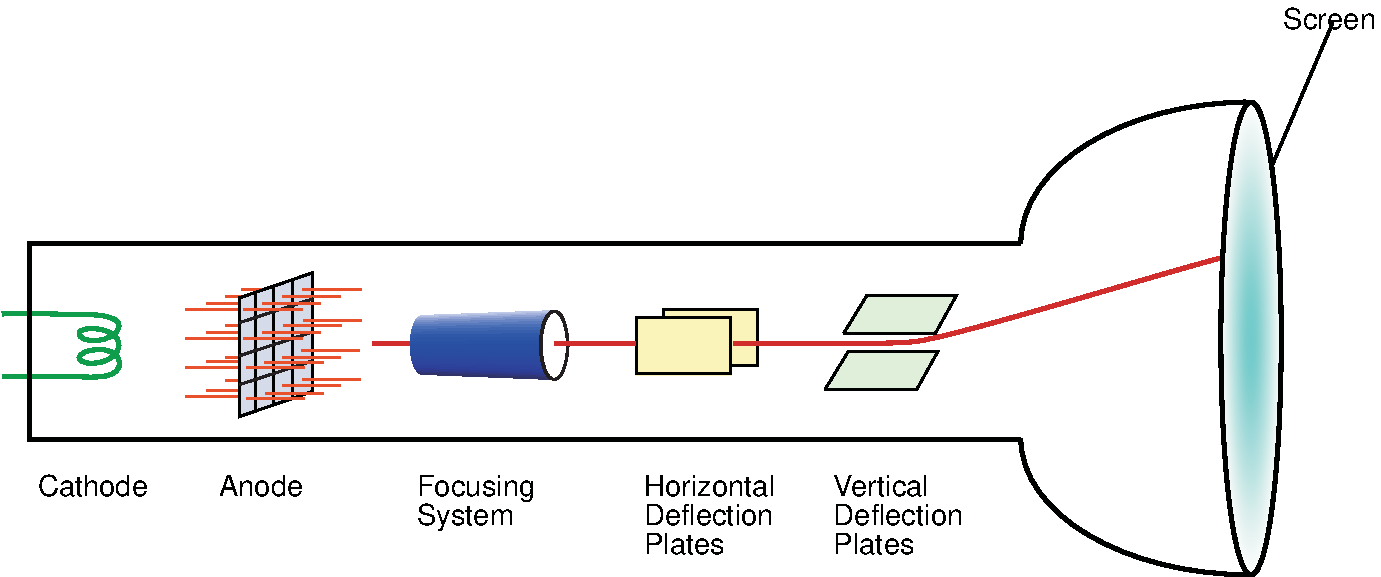
\includegraphics[width=\textwidth]{ch-physical/crt}}
\caption{Schematic diagram of a CRT.\label{fg:crt}}
\end{figure}

The two most prevalent computer displays are \emph{cathode ray tubes}
(CRTs) and \emph{liquid crystal displays} (LCDs); we'll just discuss
\index{CRT|(}
\index{LCD}
CRTs here (while they are becoming rarities, their operation is more
accessible for our purposes here). A simplified CRT is sketched in
figure~\ref{fg:crt}. It is
composed of an \emph{electron gun}, which generates \emph{cathode
\index{CRT!electron gun|(}
rays} (aka, ``electrons''). In this gun, a metal cathode is heated to
\index{CRT!cathode}
\index{CRT!cathode rays}
cause electrons to ``boil off;'' they are accelerated toward the
screen by a positively-charged anode (or possibly by charging the
\index{CRT!anode}
screen itself), which attracts the negatively-charged electrons. In
between the anode and the cathode is a negatively-charged control
grid. By varying the charge on the control grid, the intensity of the
beam can be varied in a manner analogous to the way that a faucet
valve controls the flow of water.

After leaving the electron gun, the flow of elecrons is focused into a
narrow beam by an electrostatic or magnetic focusing system. The
focused beam then passes by deflection plates, which can ``steer'' the
beam magnetically to hit any part of the screen.
\index{CRT!electron gun|)}

The screen itself is coated with one (for B\&W) or more (for color)
\emph{phosphors}: chemicals which glow (emit visible light) when struck
\index{CRT!phosphor}
by electrons. Different phosphors emit different light wavelengths,
and so multiple phosphors can be used to produce the perception of
color images (typically by combining red, green, and blue
phosphors). Another property of phosphors is \emph{persistence}: how
long it will glow after an impinging electron beam is removed. Low
persistence phosphors will require that the screen image be
\emph{refreshed} more often (by repainting the screen with the
electron beam); otherwise, the display will flicker. On the other
hand, a high persistence phosphor will glow longer, and so will
produce blurry moving images.

\begin{figure}
\centerline{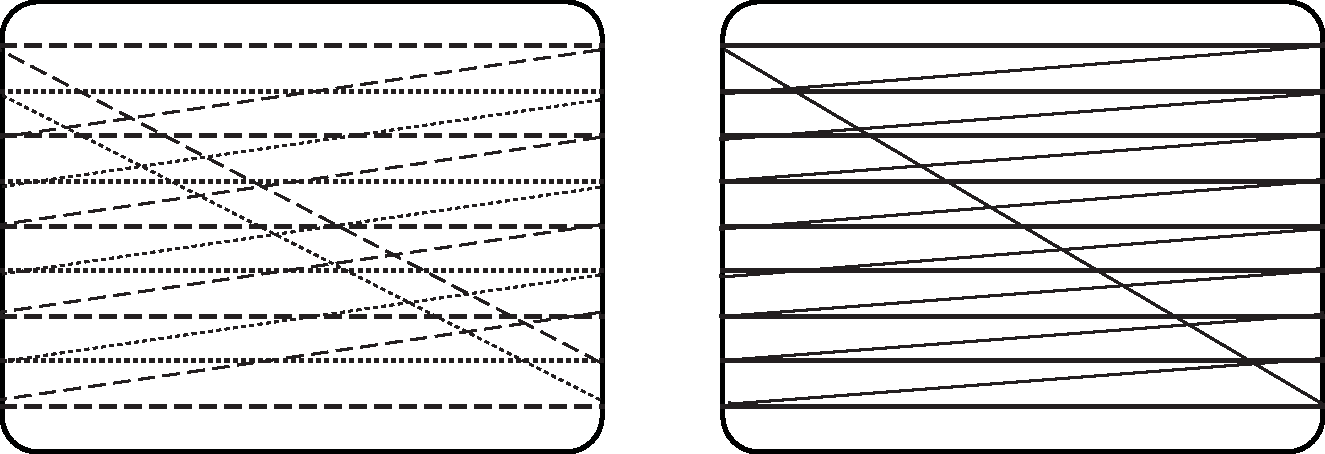
\includegraphics[width=\textwidth]{ch-physical/raster}}
\caption[Interlaced and non-interlaced raster 
  scanning]{Interlaced (left) and non-interlaced (right) raster
  scanning.\label{fg:raster}}
\end{figure}

\index{CRT!raster scanning|(}
So, how can we ``paint'' a two-dimensional image with an electron beam
that only creates a single spot on the screen? We do this by
\emph{raster scanning} the beam, as shown in
figure~\ref{fg:raster}. The horizontal and vertical deflection systems
work in concert with the control grid to move the beam across the
screen while varying its intensity. When the beam moves across the
screen horizontally, its intensity is varied in proportion to the
desired light intensity. While the deflection system resets to the
beginning of the next horizontal line, the beam is turned off. This is
called \emph{horizontal retrace}.

Subsequent lines are painted on the display in a similar manner until
the bottom of the screen is reached --- this is one \emph{frame}. At
that point, the beam is turned off and the deflection system resets
itself to the beginning of the top screen line; a process called
\emph{vertical retrace}.

For computer displays, a frame is usually displayed in between 1/60
and 1/80 of a second (though some displays have higher refresh
rates). Typically, such displays are non-interlaced
\index{CRT!raster scanning!non-interlaced}
(figure~\ref{fg:raster}, right). Analog televisions, on the other
hand, have interlaced displays (left). Interlaced raster scanning
\index{CRT!raster scanning!interlaced}
involves painting all of the odd scan lines in about 1/60 of a second,
then a vertical retrace, and a painting of the even lines.  This
allows the TV 1/30 of a second to display an entire frame and yet
still presents a flicker-free image (because every other line is
refreshed every 1/60 of a second).
\index{CRT!raster scanning|)}

\index{CRT!color|(}
This explains how a greyscale display works. But, what about color? A
color display requires three different phosphors, usually considered
to be red, green, and blue (RGB). In color monitors, three electron
guns are used --- one dedicated to each color. The guns are aligned so
that their beams strike slightly different spots on the screen. The
three phosphors are laid down in a pattern so that each color gun's
beam will hit the appropriate phosphor for each pixel. By varying the
intensity of each beam appropriately, control of the relative mix of
the three primary colors (and thus the perceived color) and the
overall brightness is possible.
\index{CRT!color|)}
\index{CRT|)}

\section{Multimedia System Operation}

\index{multimedia systems!basic functions|(}
Multimedia systems need to support four basic functions:

\begin{enumerate}
\item They must support appropriate user \emph{perception} of the
media --- provide output media and represent (code) media in such a
way that the output seems natural.
\item They must be able to \emph{retain} media --- store it and
provide efficient access (perhaps in a database).
\item They should allow users to \emph{reason} about media
information.  If the goal is greater than a digital television or
radio, then users must be able to manipulate the media.
\item They must be capable of \emph{transmitting} media between
machines. This can have significant impact on networking, resource
allocation, and synchronization of activity across geographically
distributed computer systems.
\end{enumerate}

\index{multimedia systems!computing requirements}
All of these place a high demand on computer power. For example, let's
assume that we encode audio information as 8 bits per sample at 8000
samples per second (this would be considered very low quality). How
many bits per second is that (answer in~\ref{sc:ch1ex}
\#\ref{it:ch1ex1})? Perhaps that doesn't sound too bad, so let's
consider video. Let's say we encode each frame in a video stream as
1000x1000 pixels, 24 bits/pixel, and 30 frames/second.  How many bits
per second is that (answer in~\ref{sc:ch1ex}
\#\ref{it:ch1ex2})?
Even if we were to achieve an extremely high compression ratio of
1/500, this would still mean more than 1 million bits/second.

On the one hand, we can attack this problem through faster
hardware. But you should be well aware by this time that the
difference between a good algorithm and a bad one can be the
difference between an application which places very little load on a
modest CPU and one which takes all the power of a supercomputer. That
is what we will be focusing on here: developing the mathematical
underpinning for developing efficient multimedia signal processing
algorithms.
\index{multimedia systems!basic functions|)}

\section{Vibrations and Sound}

For much of this book, we will focus on sound when talking about
signals. The reason we do this is that sound is simpler than
video. Sound is a one-dimensional function of time (amplitude versus
time), while video is at least a three-dimensional function of time
(intensity at each $x$ and $y$ pixel location as a function of time
for greyscale; R, G, B values at each $x$ and $y$ pixel location as a
function of time for color).

Sound is carried by pressure waves in the air. These pressure waves can be generated by a variety of different sources. Ideally, the human ear responds to anything that vibrates between about 20 Hz and 20 kHz. A stereo speaker in a home theater system generates sound by vibrating a flexible cone. The human vocal tract generates sound by rapidly opening and closing a muscle called the glottis as air passes through it from the lungs. Musical instruments resonate at specific frequencies depending on the width and length of strings or pipes.

In nature, sound is the result of a chaotic mix of events. It may at first seem surprising, then, that most sounds occurring in nature \emph{repeat} (usually hundreds or thousands of times per second). Figure \ref{fg:periodicexample} shows graphs of sounds generated from a tuning fork and the vocal tract (the sound `a' like in bat). In each case notice that the some portion of the wave repeats; repeating signals are commonly called \emph{periodic}. This phenomenon has spurred scientists and mathematicians to develop standard means of representing periodic signals. 
\begin{figure}
\centerline{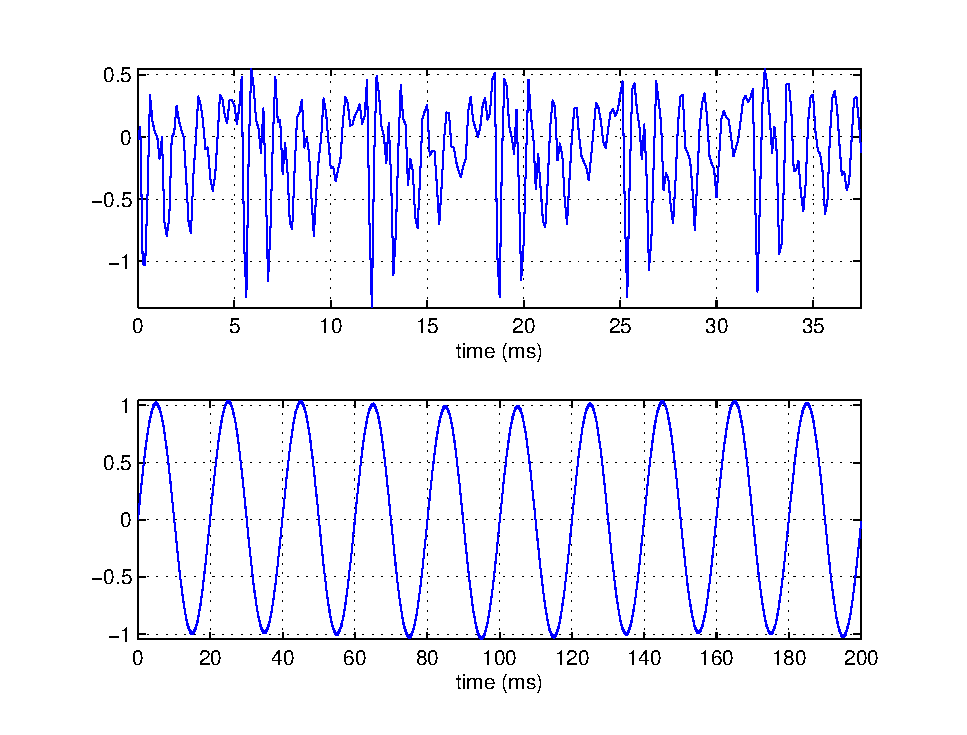
\includegraphics[width=\textwidth]{ch-physical/periodic-examples}}
\caption[Real periodic signals]{Real periodic signals. Top: human speech of the vowel `a' as in `bat.' Bottom: ringing of a tuning fork. \label{fg:periodicexample}}
\end{figure}

As we will see, it turns out that any periodic signal can be
represented as a weighted sum of \emph{harmonically} \index{harmonics}
related sines and cosines (sinusoids at frequencies that are integer
multiples of each other). If a periodic signal has a period of $T_0$
(where period is merely the reciprocal of frequency, so $T_0 =
1/f_0$), it can be represented by a weighted sum of sinusoids at
harmonics of $T_0$, namely sinusoids with periods of $T_0$,
$\frac{1}{2}T_0$, $\frac{1}{3}T_0$, $\frac{1}{4}T_0$, $\cdots$. This
is potentially very powerful! It means that if we know the period of
any repeating function, we can represent it by a discrete set of
weights (one weight for each harmonic).

Each weight tells us exactly how much to multiply by each harmonic, and thus, how much of a certain frequency is present in a given signal. By graphing the weights of each harmonic versus the frequency, we can analyze the frequency content of the signal. This is commonly known as the Fourier Series (we will discuss this later). 

The reason sines and cosines occur so often in nature is due to the physics of the way objects vibrate. When an object is acted on by a force, the way the object moves (its displacement) is a function of its velocity and acceleration. When solving for the exact displacement equation, $x(t)$, we often end up with an equation of the form,

\begin{equation}
\sderiv{x(t)}{t} = -C x(t) \label{eq:diffeq1}
\end{equation}
\index{differential equations}
where C is some constant and $\sderiv{x(t)}{t} $ is the acceleration of the object. This kind of equation --- which relates a derivative of
something to itself --- is called a \emph{differential equation}. We
bet you didn't know they were that simple! To \emph{solve} a
differential equation, we look for a function, $x(t)$, that will satisfy the equation. This is analogous to
solving an algebraic equation, where we look for a number that
can be substituted for a given variable.  
The only difference is that numbers fall along a
one-dimensional number line (unless we're talking about complex
numbers), while there is no such neat number line for all possible functions.  So, we
need to find a function, $x(t)$, whose second derivative is proportional
to itself. Can you think of one or two (answer in~\ref{sc:ch1ex}
\#\ref{it:ch1ex3})?

Luckily, people have been working with functions and differential
equations for a while, and so finding such functions is not
difficult.  For example, consider sinusoids.  The first and second
derivatives of $\sin\omega t$ are:

\begin{gather}
\deriv{}{t} \sin\omega t = \omega\cos\omega t\\
\sderiv{}{t} \sin\omega t = \deriv{}{t} \omega\cos\omega t\
   = -\omega^2 \sin\omega t
\end{gather}

Therefore, differential equation~(\ref{eq:diffeq1}) describes
\emph{simple harmonic motion}: sinusoidal vibration of a simple object. 
Sinusoids occur naturally in the real world when an object is acted on by a force! More complicated forces and objects result in more complicated differential equations, but they almost always involve sines and cosines.

%\index{tuning fork|(}
%As I said earlier, sound is carried by pressure waves in the air. such
%pressure waves can be generated by vibrating a physical object.  For
%example, a speaker generates sound by vibrating a flexible cone. Let's
%start with a simple vibrating system: a tuning fork producing a pure
%tone. And, to make things even simpler, we'll consider only a
%single-tine fork (a tuning chopstick?).
%
%\begin{figure}
%\centerline{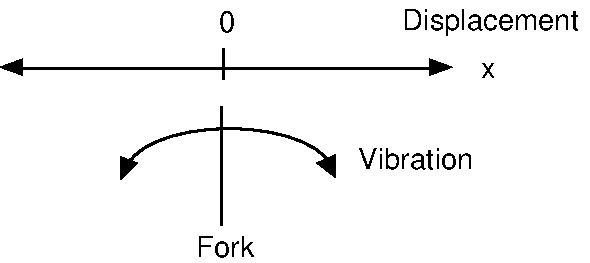
\includegraphics[width=\textwidth]{ch-physical/tuningfork}}
%\caption{Vibration of an idealized tuning fork.\label{fg:tuningfork}}
%\end{figure}
%
%There are three concepts central to our understanding of how the
%idealized tuning fork in figure~\ref{fg:tuningfork} vibrates:
%\begin{description}
%\item[deformation] The fork is assumed to be fixed at one end and free
%  at the other, which swings back and forth as the fork vibrates. So,
%  the material the fork is made of is \emph{bent} as the end swings.
%\item[inertia] An object (such as the end of the vibrating fork)
%  exerts a force proportional to its mass when one tries to accelerate
%  or decelerate it. We can write the equation for this force as $F_i =
%  ma$, where $F_i$ is the inertial force, $m$ is the object's mass,
%  and $a$ is the acceleration.
%\item[elastic forces] Deforming the fork requires application of
%  force.  In the case of our tuning fork, the force results from its
%  inertia. Let's make the simplifying assumption that the fork acts
%  like an ideal spring. That means that as the fork is bent from the
%  vertical ($x=0$ in the figure), the elastic force increases
%  proportionately to $x$. So, $F_e = -kx$, where $F_e$ is the elastic
%  force, $k$ is the spring constant (how stiff the fork is), and the
%  minus sign indicates that the direction of the force is opposite the
%  directio of the bend (always towards $x=0$).
%\end{description}

%So, we pull the fork and release it.  The elastic force results in an
%acceleration towards $x=0$ and the tip speed builds up.  When the tip
%passes $x=0$, the elastic force decelerates the tip, it stops, and the
%whole thing repeats. If we ignore troublesome issues like air
%resistance that would slow down the vibration, then $F_i = F_e$.
%Solving for $a$ we obtain:
%
%\begin{align}
%F_i = ma &= -kx = F_e \\
%a &= -\frac{k}{m} x
%\end{align}
%
%Acceleration is the change in velocity over time, or its derivative,
%$a = \mathrm{d}v/\mathrm{d}t$; velocity in turn is the derivative of
%distance, $v = \mathrm{d}x/\mathrm{d}t$. So, acceleration is the second
%derivative of $x$:
%
%\begin{equation}
%a = \deriv{v}{t} = \sderiv{x}{t} = -\frac{k}{m} x \label{eq:tuningfork}
%\end{equation}
%
%\index{differential equations}
%As an aside, this kind of equation --- which relates a derivative of
%something to itself --- is called a \emph{differential equation}. I'll
%bet you didn't know they were that simple! To \emph{solve} a
%differential equation, we look for a function of $x$ that, when
%plugged in for $x$, will satisfy the equation. This is analogous to
%solving an algebraic equation, where we look for a number that
%satisfies.  The only difference is that numbers fall along a
%one-dimensional number line (unless we're talking about complex
%numbers), while there is no such neat ordering of functions.  So, we
%need to find a function of $x$ whose second derivative is proportional
%to itself. Can you think of one or two (answer in~\ref{sc:ch1ex}
%\#\ref{it:ch1ex3})?
%
%Luckily, people have been working with functions and differential
%equations for a while, and so finding such functions is not
%difficult.  For example, consider sinusoids.  The first and second
%derivatives of $\sin\omega t$ are:
%
%\begin{gather}
%\deriv{}{t} \sin\omega t = \omega\cos\omega t\\
%\sderiv{}{t} \sin\omega t = \deriv{}{t} \omega\cos\omega t\
%   = -\omega^2 \sin\omega t
%\end{gather}
%
%Therefore, differential equation~(\ref{eq:tuningfork}) describes
%\emph{simple harmonic motion}: sinusoidal vibration of the tuning
%fork's tip.
%\index{tuning fork|)}
%
%\subsection*{Self-Test Exercises}
%
%See~\ref{sc:ch1ex} \#\ref{it:ch1ex4}--\ref{it:ch1ex5} for answers.
%
%\begin{enumerate}
%\item Solve for $\omega$ in terms of $k$ and $m$.
%\item Fork stiffness ($k$) clearly affects vibration frequency. As the
%  fork get stiffer ($k$ increases), does the vibration frequency go up
%  or down?
%\end{enumerate}

\subsection*{Sinusoid Phase}

Because sines and cosines are so powerful it is necessary to represent them as neatly and compactly as possible. Above we saw why $\sin\omega t$ occurs naturally. The same argument can be used for $\cos\omega t$.  In fact, cosine is
just a delayed version of sine, as $\cos\omega t = \sin(\omega t +
\pi/2)$.  So, a more general solution to~(\ref{eq:diffeq1}) would
be:
\begin{equation}
x(t) = \sin(\omega t + \phi) \label{eq:gensine}
\end{equation}

\index{phase!of a sinusoid}
In~(\ref{eq:gensine}), $\phi$ is called the sinusoid's \emph{phase}:
the time closest to $t=0$ when $x(t)=0$ (for the case of a sine; it
would be when $x(t)=1$ for a cosine). Depending on \emph{when} an object
starts vibrating (and our time reference; the time that we call $t=0$),
we will get sinusoids of differing phase.

Let's use tuning forks as an example. 
What would happen if we hit two identical tuning forks but at
different times?  They would vibrate at the same frequency, but would
have differing phases and amplitudes (loudnesses).  If the two forks
were close together, we would hear the sum of their tones. What would
that sum be (answer in~\ref{sc:ch1ex} \#\ref{it:ch1ex6})? Simplifying
this sum would be involved; we would have to remember all sorts of
trigonometric identities and then crank out the algebra. Luckily, we
can come up with another representation of a sinusoid which simplifies
this problem considerably. In fact, much of the new math we will cover
in this course is primarily focused on making the paper-and-pencil
work easier.

\section{Phasors}

\begin{figure}
\centerline{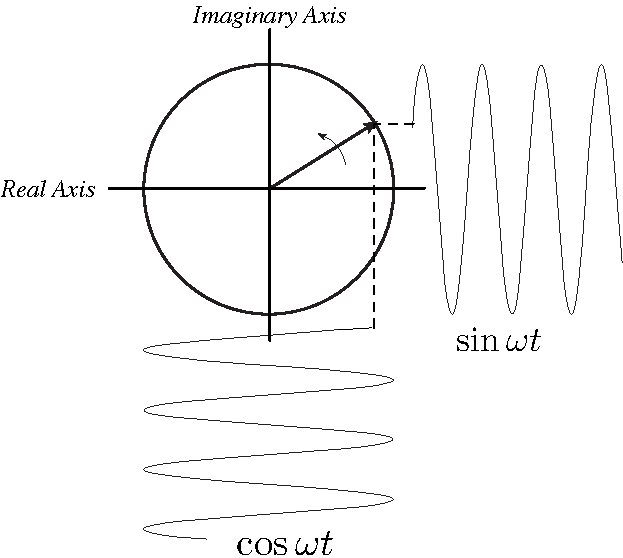
\includegraphics[width=0.5\textwidth]{ch-physical/phasor-components}}
\caption{Components of a phasor are sinusoids.\label{fg:phasor-components}}
\end{figure}

Instead of thinking of a sinusoid as a function which oscillates up
and down, let's think of it as something that goes round and round: a
rotating vector of length $a$ (where $a$ is the sinusoid's
amplitude). Think of this vector rotating around the origin of the
$x$-$y$ plane.  At any point in time, the vector makes an angle
$\theta(t)$ with the positive $x$ axis. The phase, $\phi$, is defined
as $\phi = \theta(0)$ (i.e., the angle that the vector makes with the
$x$-axis at $t=0$).  As figure~\ref{fg:phasor-components} shows, the
$x$ and $y$ \emph{components} of the vector as it moves
counterclockwise are cosine and sine functions.

If we have two vectors $\mathbf{u}$ and $\mathbf{v}$, we can add them
by adding their components.  This is done graphically in
figure~\ref{fg:vector-sum} by placing the ``tail'' of one vector on
the ``head'' of the other. The sum $\mathbf{u}+\mathbf{v}$ is the
vector from the origin to the ``head'' of the second vector. Of
course, that's just the sum at one point in time. What does
$\mathbf{u}+\mathbf{v}$ look like if $\mathbf{u}$ and $\mathbf{v}$ are
rotating at the same rate (answer in~\ref{sc:ch1ex} \#\ref{it:ch1ex7})?

\begin{figure}
\centerline{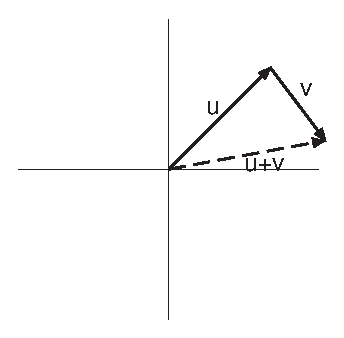
\includegraphics[width=0.5\textwidth]{ch-physical/vector-sum}}
\caption{Graphical summation of vectors.\label{fg:vector-sum}}
\end{figure}

\subsection*{Complex Exponential Representation}

While we used the $x$ and $y$ axes above as frames of reference (for
considering components --- sine and cosine --- of the vector), we
didn't actually define what the plane was. Let's imagine that our
rotating vectors are in the \emph{complex} plane, where $x$ is the
real axis and $y$ is the imaginary axis.  At any point in time, the
location of a vector is therefore a complex number: \index{complex
  numbers|(emph}

\begin{equation}
\mathbf{v} = x + j y \label{eq:complexrect}
\end{equation}

\index{j ($\sqrt{-1}$)}
\index{i|see{j}}
We use $j$ here for $\sqrt{-1}$, rather than $i$ as you've probably
seen before, to adhere to the convention used by electrical engineers
(who use $i$ for current). This notation allows us to represent vectors in the complex plane as complex numbers.

\index{complex numbers!rectangular form}
\index{complex numbers!polar form}
\index{complex numbers!magnitude|see{complex numbers, polar form}}
\index{complex numbers!angle|see{complex numbers, polar form}}
Note that equation \ref{eq:complexrect} is the \emph{rectangular} representation of complex
numbers; we can also represent them in polar form (magnitude and
angle), written as $R\angle\theta$. 


\problemset{
\subsubsection*{Review Exercises: Complex Numbers}
\begin{enumerate}
\item What is the sum of the two complex numbers $x + jy$ and $v +
  jw$ (answer in~\ref{sc:ch1ex} \#\ref{it:ch1excn1})?
\item What is the
product of the two complex numbers $x + jy$ and $v +
  jw$ (answer in~\ref{sc:ch1ex} \#\ref{it:ch1excn2})?
\item Convert the complex number $z = x + jy$ to polar form,
  $R\angle\theta$ (answer in~\ref{sc:ch1ex} \#\ref{it:ch1excn3}).
\item Multiply the two polar-form complex numbers $R_1\angle\theta_1$ and
  $R_2\angle\theta_2$ (answer in~\ref{sc:ch1ex} \#\ref{it:ch1excn4}).
\end{enumerate}
\index{complex numbers|)}}

So, we have an easier-to-manipulate representation of a vector
\emph{at one point in time}. But, we want to represent a \emph{rotating}
vector.  Let's talk about a ``standard'' sinusoid --- one with unit
amplitude --- and let's call this $E(\theta)$.  We know from our first
discussion of the rotating vector representation that cosine and
sine are the $x$ and $y$ axis projections of the vector, so let's
rewrite our rectangular form in the complex plane as:

\begin{equation}
E(\theta) = \cos\theta + j\sin\theta \label{eq:cmplx-sin-rect}
\end{equation}

Can we rewrite the polar form in a similar way? We need
a function of $\theta$ that satisfies the same requirements as the
rectangular form of equation~(\ref{eq:cmplx-sin-rect}). The derivative
of~(\ref{eq:cmplx-sin-rect}) is:

\begin{equation}
\deriv{}{\theta} E(\theta) = -\sin\theta + j\cos\theta
\label{eq:cmplx-sin-ddt}
\end{equation}

We note that~(\ref{eq:cmplx-sin-ddt}) is also just $jE(\theta)$, which
is the original function times a constant. What function satisfies the
condition that its derivative is proportional to itself? 

\begin{align}
E(\theta) &=  e^{j\theta} \\ \label{eq:cmplx-sin}
\deriv{}{\theta} E(\theta) &=  je^{j\theta}
\end{align}

This is the \emph{complex exponential} representation. It has the
property that $e^{j\theta} = \cos\theta + j\sin\theta$; also called
\emph{Euler's formula} (``Euler'' is pronounced ``oiler''). It will
\index{Euler's formula|emph} make our work much simpler.  For
example, \emph{raising the complex exponential to a power is equivalent
to rotating the vector}:

\begin{equation}
E(\theta)^k = \left( e^{j\theta} \right) ^k
            = e^{j\theta} e^{j\theta} \cdots e^{j\theta}
            = e^{jk\theta} \label{eq:pow-rot}
\end{equation}

As you can see in~(\ref{eq:pow-rot}), raising $E(\theta)$ to the
$k^{\textrm th}$ power is equivalent to multiplying the angle $\theta$
by $k$ in the complex exponential.

The complex exponential $e^{j\theta}$ has unit
magnitude.  The representation for a general complex vector $R\angle\theta$
is therefore $Re^{j\theta}$. So, we see that the sine and cosine
representation is the rectangular form, and the complex exponential is
the polar form.

\begin{align} \centering
	E(\theta) &= Re^{j\theta} && \text{(polar form)} \\
	E(\theta) &= R\cos\theta+jR\sin\theta && \text{(rectangular form)}
\end{align}

\problemset{
\subsubsection*{Self-Test Exercises}
\begin{enumerate}
\item Multiply the two complex sinusoids $z_1$ and
  $z_2$ (answer in~\ref{sc:ch1ex} \#\ref{it:ch1exce1}).
\item The complex conjugate is indicated by $z^*$. If $z=x+jy$,
  $z^*=x-jy$.  What is the complex conjugate of the complex sinusoid,
  $z=Re^{j\theta}$ (answer in~\ref{sc:ch1ex} \#\ref{it:ch1exce2})?
\item Answer the following for $z = x + jy$ (answers in~\ref{sc:ch1ex}
\#\ref{it:ch1exce3}):
\begin{enumerate}
\item What is $z + z^*$?
\item What is $z - z^*$?
\item What is $zz^*$?
\end{enumerate}
\end{enumerate}}

Going back to~(\ref{eq:pow-rot}), we can now write an expression for a
\emph{complex sinusoid} as a function of time (a rotating complex exponential). The angle
of the sinusoid is a function of time, $\theta(t) = \omega t$, where
$\omega$ is its frequency (just as for our original sinusoids):

\begin{equation}
e^{j\theta(t)} = e^{j\omega t} \label{eq:phasor-first}
\end{equation}

This rotating complex sinusoid is called a \emph{phasor} (with
apologies to Captain Kirk). The phasor representation is extremely powerful. Just as with sines and cosines, it turns out that \emph{any periodic function can be written as a unique sum of phasors}. Notice that phasors are complex functions but that we can add them in special ways to represent completely real functions. For example,

\begin{align*}
f(t) &= e^{j\omega t}+e^{-j\omega t} \\
&=\cos\omega t + j\sin\omega t +\cos-\omega t + j\sin-\omega t &&\text{Use Euler's formula} \\
&=\cos\omega t + j\sin\omega t +\cos\omega t - j\sin\omega t &&\text{simplify $-\omega$} \\
&= 2\cos\omega t
\end{align*}
where we have used odd and even symmetry properties of sinusoids, ($\sin-x=-\sin x$) and ($\cos-x=\cos x$). The function $f(t)$ was represented as a sum of complex exponentials but had no imaginary component! In fact, sinusoids are often represented using complex exponentials.

\begin{align}
\cos x &= \frac{e^{jx}+e^{-jx}}{2}\\ 
\sin x &= \frac{e^{jx}-e^{-jx}}{2j}
\end{align}


\subsection*{Practical Example: Tuning a Guitar}

When a person tunes a guitar, they usually tune just the lowest string
to a reference (a pitch pipe, for example). Then, they finger that
string to produce the same note that the next higher string should.
If the second string does produce the same tone, they can hear that.
If the second string is out of tune, it will produce a slightly
different tone, and they can hear \emph{beating}. Beating is what
results when two sinusoids at different frequencies are added.

Previously, we added two sinusoids at the same frequency, and saw that
the result is another sinusoid at that same frequency.  That is the
case when the second string is in tune. Let's now add two complex
sinusoids with slightly different frequencies, $\omega$ and $\omega +
\delta$, where the difference between the two frequencies is
$\delta\ll\omega$:

\begin{align}
a_1 e^{j\omega t} + a_2 e^{j(\omega+\delta)t} &=
   a_1 e^{j\omega t} + a_2 e^{j\omega t} e^{j\delta t} \notag \\
 & = \underbrace{(a_1 + a_2 e^{j\delta t})}_\mathrm{low~frequency} 
        \underbrace{e^{j\omega t}}_\mathrm{high~frequency} 
\end{align}
  
\begin{figure} 
\centerline{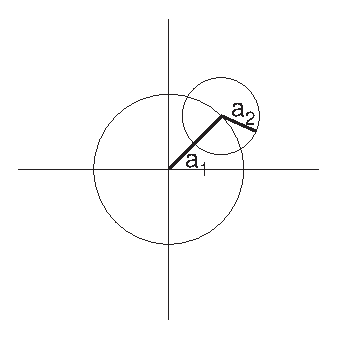
\includegraphics[width=0.5\textwidth]{ch-physical/beating}}
\caption{Phasor representation of beating.\label{fg:beating}} 
\end{figure} 

\begin{figure} 
\centerline{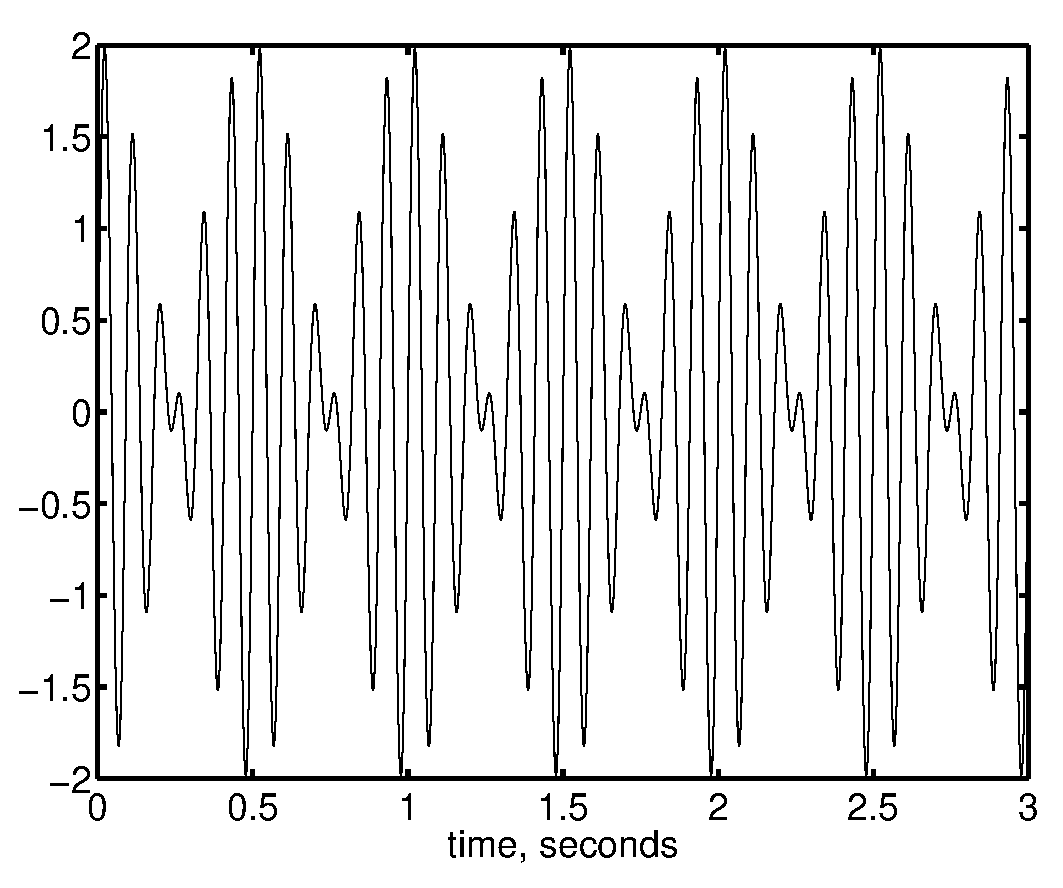
\includegraphics[width=0.5\textwidth]{ch-physical/beating-waveform}}
\caption{Amplitude vs. time representation of beating.\label{fg:beating-waveform}} 
\end{figure} 

This has the form of a complex sinusoid of frequency $\omega$ and
amplitude that is a function of time, $a_1 + a_2 e^{j\delta t}$, that
varies with a frequency of $\delta$. Figure~\ref{fg:beating} presents
the graphical version of this, which looks like a top view of the
amusement park ``octopus'' ride. There are times when the $e^{j\delta
  t}$ adds a factor of up to $a_2$ to the first sinusoid and times
when it subtracts a factor of up to $a_2$. The result is the beating
waveform seen in figure~\ref{fg:beating-waveform} (in this case, the
result of adding 10Hz and a 12Hz sinusoids, which can be seen to
produce a 2Hz ``beat frequency'').

\problemset{
\subsubsection*{MATLAB and Sound Files}
\begin{sloppypar}
\begin{itemize}
\item A MATLAB .m file for demonstrating beating is available at
\url{http://faculty.washington.edu/stiber/pubs/Signal-Computing/beating.m}.
\index{MATLAB code!beating}
\item Audio files to demonstrate beating: a 1000Hz
sine wave at
\url{http://faculty.washington.edu/stiber/pubs/Signal-Computing/1000Hz.au}, a 1005Hz
sine
wave at \url{http://faculty.washington.edu/stiber/pubs/Signal-Computing/1005Hz.au}, and
their
sum, at \url{http://faculty.washington.edu/stiber/pubs/Signal-Computing/beating.au}.
\index{audio files!beating}
\index{sound files|see{audio files}}
\end{itemize}
\end{sloppypar}}

\subsection*{Frequency and Period}

\index{frequency!angular}
\index{$\omega$}
\index{frequency!Hertz (Hz)}
Until now, we've been using $\omega$ as the symbol for the speed of
rotation of a phasor. If $t$ is in seconds (which we will assume is
always the case), then the phasor rotates $\omega/2\pi$ times in one
second, or once in $2\pi/\omega$ seconds. Remembering that our
exponential representation corresponds $\cos \omega t + j \sin \omega
t$, we see that each of these rotations corresponds to $2\pi$ radians
in the oscillation of a sinusoid, and so its units must be
\emph{radians/second}. We will call this \emph{angular frequency}, as
it is the rate of change of the phasor's angle per second. However,
when we speak of periodic physical signals, it is more convenient to
speak of the number of times that the signal repeats per second:
\emph{cycles/second} or \emph{Hertz}. We will use $f$ to refer to
frequencies expressed as Hertz. Since one cycle is $2\pi$ radians, we
can convert between these two units as $\omega = 2\pi f$. In this
book, we will use whichever units are most convenient for each topic;
you'll need to note which is in use.

\index{period!of a sinusoid}
If $\omega$ and $f$ are the number of radians or cycles of a sinusoid
per second, then their reciprocals are the number of seconds per
radian or cycle of rotation. Seconds per radian is only infrequently
used, so we only define a symbol for seconds per cycle, $T = 1/f =
2\pi/\omega$. This is the \emph{period} of a signal in seconds.

\section{Spectra}

Let's return to our discussion of \emph{harmonics}, but now using complex exponentials. We stated earlier that any periodic function could be represented by a sum of weighted harmonics. Let's start with a sum of two sinusoids.
\index{harmonics}
Let's call the first sinusoid's frequency $\omega_0$ and the second's
$\omega_1 = m\omega_0$, $m=2, 3, \ldots$. Their sum is $a_0
e^{j\omega_0 t} + a_1 e^{jm\omega_0 t}$, and there's nothing we can do
to simplify this equation. This ``failure to simplify'' is not a
result of our lack of mathematical sophistication --- there truly is
no simpler representation. Another way of saying this is that
sinusoids at different frequencies are independent or
\emph{orthogonal} to each other. %
\index{sinusoids!orthogonal}%
\index{sinusoids!independent}%
\index{orthogonality}%
\index{independence}%
In general, if we add a large number
of harmonics together, their sum is:
\begin{equation}
\sum_{k=0}^N a_k e^{jk\omega_0 t}
\label{eq:sum-harmonics}
\end{equation}

You'll note that the $k=0$ term of this summation has the value $a_0$
for all time; this is often called the \emph{DC component} of the
\index{DC component}
signal. All other components have frequencies that are integer
multiples (harmonics) of $\omega_0$, the \emph{fundamental
frequency}. Note that a sinusoid with frequency $k\omega_0$ has a
\index{frequency!fundamental}
period of $2\pi/(k\omega_0) = T_0/k$ --- it repeats $k$ times in $T_0$
seconds. This means it \emph{also repeats} every $T_0$ seconds, and since
each term in the summation repeats every $T_0$ seconds, the whole
summation repeats that often, and therefore the period of the signal
represented by the summation is $T_0$. As we said before, such
a summation can in fact be used to represent \emph{any} periodic
function of time. The series of weights, $a_k$, is known as the \emph{Fourier Series}. This \emph{Fourier series} is one of the most
\index{Fourier series|emph}
important and fundamental principles of signal processing. It allows us to look at the \emph{spectrum} of a signal.

\index{spectrum}
You should be familiar already with the term ``spectrum'' as used to
describe the continuous band of colors that white light (sunlight) can
be broken into --- a rainbow. From physics, you know that each color
corresponds to a specific frequency of the visible spectrum. Hence,
the decomposition of white light into colors is actually a form of
frequency analysis. \emph{Frequency analysis} involves the
\index{frequency analysis}
decomposition of a signal into its frequency (sinusoidal) components;
this is also called \emph{spectral analysis}. The multimedia signal
\index{spectral analysis}
waveforms we are concerned with here are basically functions of
time.

At this point, you should recognize that the Fourier series represents
the spectrum of a periodic signal.  It (and other tools) decomposes
signals into spectra defined in terms of sinusoidal (or complex
exponential) components. With such a decomposition, a signal is said
to be represented in the
\emph{frequency domain}; otherwise, usually it is in the \emph{time
domain}. For periodic signals, such a decomposition is the Fourier
Series. For infinite signals (with finite energy), the decomposition
is called a \emph{Fourier Transform}. For finite, discrete signals,
the decomposition is the \emph{Discrete Fourier Transform}.
Recombining the sinusoidal components to reconstruct the original
signal is basically a Fourier synthesis problem or
\emph{inverse Fourier analysis}. 

The weights, $a_k$, of the Fourier Series are usually complex valued. To explain the derivation of the Fourier Series, we therefore need to look at \emph{vectors} in the complex plane.

%%%
%\index{z-transform!properties of}
%\begin{table}
%\caption{Some properties of the z-transform.\label{tb:zt-property}}
%\begin{center}
%\begin{tabular}{|l|c|c|} \hline
%Property      & Time Domain, $Z^{-1}\{\cdot\}$ & z-Domain, $Z\{\cdot\}$ \\ \hline\hline
%Linearity     & $a_1x[n]+a_2y[n]$ & $a_1X(z)+a_2Y(z)$\\ 
%Time shift    & $x[n-k]$       & $z^{-k}X(z)$\\ 
%Scaling in the z-domain 
%              & $a^nx[n]$        & $X(a^{-1}z)$ \\ 
%Time reversal & $x[-n]$        & $X(z^{-1})$\\ 
%Differentiation in the z-domain 
%              & $nx[n]$          & $-z \deriv{X(z)}{z}$ \\ 
%Convolution   & $x[n] \ast y[n]$       & $X(z)Y(z)$ \\ \hline
%\end{tabular}
%\end{center}
%\end{table}
%%%
\subsection{Interlude: Vectors}

\index{vectors|(}
Here is a list of vector operations, most of which you are likely already familiar with. Let $\mathbf{v}$ and $\mathbf{w}$ be arbitrary vectors and
$\vec{\mathbf{x}}, \vec{\mathbf{y}}$ and $\vec{\mathbf{z}}$ be an
orthogonal \emph{basis} (the component vectors that define the
\index{vectors!basis}
coordinate system, which for 3D Cartesian coordinates would be unit
vectors parallel to the $X$, $Y$, and $Z$ axes).  We can then define
the following:

\begin{enumerate}
\item Projection of a vector onto the basis vectors (you may
know these as the \emph{components} of the vector)
\index{vectors!projection}
\index{vectors!components}
\begin{align}
v_x &= \langle\mathbf{v},\vec{\mathbf{x}}\rangle \notag\\
v_y &= \langle\mathbf{v},\vec{\mathbf{y}}\rangle \label{eq:basis-proj}\\
v_z &= \langle\mathbf{v},\vec{\mathbf{z}}\rangle \notag\\ 
\end{align}
and 
\begin{align}
w_x &= \langle\mathbf{w},\vec{\mathbf{x}}\rangle \notag\\
w_y &= \langle\mathbf{w},\vec{\mathbf{y}}\rangle \\
w_z &= \langle\mathbf{w},\vec{\mathbf{z}}\rangle \notag\\ 
\end{align}
\item Expressing a vector using the basis (i.e., as the sum of its
components)
\index{vectors!as sum of components}
\begin{align}
\mathbf{v} &= v_x\vec{\mathbf{x}} + v_y\vec{\mathbf{y}} +
v_z\vec{\mathbf{z}} \label{eq:vec-comps}\\ 
\mathbf{w} &= w_x\vec{\mathbf{x}} + w_y\vec{\mathbf{y}} +
w_z\vec{\mathbf{z}}
\end{align}
\item Inner product of two vectors
\index{vectors!inner product}
\begin{align}
\langle\mathbf{v}, \mathbf{w}\rangle &= v_xw_x +  v_yw_y + v_zw_z
 \label{eq:inner-product}\\
\langle\mathbf{v}, \mathbf{v}\rangle &= v_x^2 +  v_y^2 + v_z^2
\end{align}
You may be familiar with the inner product of a vector with itself as
being its length squared, $|\mathbf{v}|^2$.  When the vector is
complex the inner product is defined as:
\begin{align}
\langle\mathbf{v}, \mathbf{w^*}\rangle &= v_xw_x^* +  v_yw_y^* + v_zw_z^*
 \label{eq:complex-ip}\\
\langle\mathbf{v}, \mathbf{v^*}\rangle &= |v_x|^2 + |v_y|^2 + |v_z|^2
\end{align}
where $^*$ denotes complex conjugate. 

We can also consider arbitrary functions to be more generalized forms
of vectors. If $f(t)$ and $g(t)$ are periodic functions of a
continuous time variable $t$ with period $T$, their inner product is
defined as
\begin{equation}
\langle f, g\rangle = \frac{1}{T}\int_0^T f(t)g^*(t) dt \label{eq:func-ip}
\end{equation}
which is normalized to one by $T$. Intuitively, you can think of this as a ``projection'' of one function onto another, or ``how much'' of of $f$ is in the same ``direction'' as $g$.

\item Vector sum
\index{vectors!sum}
\begin{equation}
\mathbf{v} + \mathbf{w} = 
    (v_x+w_x)\vec{\mathbf{x}}
  + (v_y+w_y)\vec{\mathbf{y}}
  + (v_z+w_z)\vec{\mathbf{z}}
 \label{eq:vec-sum}
\end{equation}
\item Distributive and commutative properties of inner products
\index{vectors!inner product!distributive property}
\index{vectors!inner product!commutative property}
\begin{align}
\langle\mathbf{v} +\mathbf{u} , \mathbf{w}\rangle &=
   \langle\mathbf{v},\mathbf{w}\rangle + \langle\mathbf{u}, \mathbf{w}\rangle
 \label{eq:ip-dist}\\
\langle\mathbf{u}, \mathbf{v}\rangle &= \langle\mathbf{v}, \mathbf{u}\rangle
 \label{eq:ip-commut}
\end{align}
\item $\mathbf{v}$ is \emph{orthogonal} to $\mathbf{w}$
\index{vectors!orthogonal}
\begin{equation}
\langle\mathbf{v}, \mathbf{w}\rangle = 0 \label{eq:orthogonal}
\end{equation}
\item Unit vector
\index{vectors!unit}
\index{unit vector}
\begin{equation}
\langle\mathbf{v}, \mathbf{v}\rangle = v_x^2 +  v_y^2 + v_z^2 =1
 \label{eq:unit-vector}
\end{equation}
\end{enumerate}
\index{vectors|)}

\subsection{Derivation of the Fourier Series}

Here we present frequency analysis tools for continuous time periodic
signals. A periodic signal is defined as: 
\begin{equation}
f(t) = f(t+T)
\end{equation}
where $t$ is a continuous time variable and $T$ is the signal's
period.

The basic mathematical representation of periodic signals is the
Fourier Series, which as we have seen is a weighted sum of
\emph{harmonically related} sinusoids (sinusoids whose frequencies are
all multiples of a single,
\emph{fundamental} one) or complex exponentials. This was first
developed in the nineteenth century by the French mathematician Jean
Baptiste Joseph Fourier to describe heat conduction. Now it has
extensive applications in a variety of problems encompassing many
different fields.

\index{Fourier Series|emph}
The \emph{Fourier Series} description of a periodic function $f(t)$, 
with period $T=2\pi/\omega_0$, is defined
as a weighted sum of complex exponentials:
\begin{equation}
f(t) = \sum_{k=-\infty}^{\infty} c_k e^{jk\omega_0 t}
\label{eq:fs}
\end{equation}
We may think of the exponential signals (or phasors)
\begin{equation}
e^{jk\omega_0 t}, \quad k = \ldots, -2, -1, 0, 1, 2, \ldots
\end{equation}
as a set of basis vectors, where $\omega_0 = 2\pi /T$ is the frequency of
the phasor in radians/second. By our earlier definition, $\omega_0$ is the
\emph{fundmental frequency}. In a Fourier series, the periodic
\index{frequency!fundamental}
function $f(t)$ is expressed in terms of the basis and $c_k$ is the
projection of $f(t)$ onto the basis $e^{jk\omega_0 t}$, just like the
projection $v_x$ of a vector $\mathbf{v}$ onto the basis $\vec{\mathbf{x}}$. The weight, $c_k$, tells us exactly ``how much'' of the signal, $f(t)$, is a result of the frequency $k\omega_0$. From
equation~\ref{eq:func-ip}, the inner product of $f(t)$ and
$e^{jk\omega_0 t}$ is
\begin{equation}
c_k = \langle f(t), e^{jk\omega_0 t}\rangle 
    = \frac{1}{T}\int_0^T f(t)e^{-jk\omega_0 t}dt.
\label{eq:fs-ck}
\end{equation}
where the \emph{Fourier coefficients} $c_k$ are called the
\index{Fourier coefficients|emph} \emph{frequency content} or
\emph{spectrum} of $f(t)$, $k=0, \pm 1, \pm 2, \ldots,
\pm\infty$. This spectrum is just like the familiar shorthand of
writing a vector as a column or row of numbers, with the understanding
that each is the coefficient of one of the basis vectors (i.e., when
we write $\mathbf{v} = [1 2 3]$, what we actually mean is $\mathbf{v}
= 1 \vec{\mathbf{x}} + 2 \vec{\mathbf{y}} + 3 \vec{\mathbf{z}}$).
This is the signal's representation in the \emph{frequency domain},
where frequency is the coordinate (in other words, the signal
expressed as a function of frequency).  Similar, $f(t)$ is the
signal's \emph{time domain} representation, where time is the
coordinate. Notice that the Fourier series transforms a finite
(periodic), continuous signal in the time domain into an infinite
(because the values of $k$ range from $-\infty$ to $+\infty$),
discrete (because $k$ only takes on integer values) spectrum in the
frequency domain.

\subsubsection{Alternative Derivation of the Fourier Series [\textsc{Optional}]}

Another way to derive the formula for the $c_k$ is as follows.  The aim of this derivation is to plug in the Fourier Series definition of $f(t)$ into the equation for $c_k$ and see if we can get exactly $c_k$ back by manipulating the equation. We
first multiply both sides of (\ref{eq:fs}) by the phasor
$e^{-jl\omega_0 t}$ ($l=\ldots, -2,-1,0,1,2,\ldots$) and then
integrate both sides of the resulting equation over a single period
[0, T],
\begin{align}
c_k=\frac{1}{T}\int_0^T f(t)e^{-jl\omega_0t}dt
&= \frac{1}{T}\int_0^T \sum_{k=-\infty}^{\infty} c_k e^{jk\omega_0t}
e^{-jl\omega_0 t}dt \notag\\
&= \sum_{k=-\infty}^{\infty} c_k \frac{1}{T}\int_0^T
e^{j(k-l)\omega_0t}dt
\label{eq:fs-ck2}
\end{align}
Note that
\begin{align}
\frac{1}{T}\int_0^T e^{j(k-l)\omega_0t}dt
&= \frac{1}{T}\left.\frac{e^{j(k-l)\omega_0t}}{j(k-l)\omega_0}
               \right|_0^T \notag\\
&= \frac{e^{j(k-l)\omega_0T} - 1}{j(k-l)\omega_0T}
    \label{eq:fs1}
\end{align}

Equation~(\ref{eq:fs1}) has two different solutions, depending on
whether $k=l$ or not. Let's make the substitution $u=k-l$. So, when
$k=l$, $u=0$, and the numerator and denominator of~(\ref{eq:fs1}) are
both zero. We therefore use L'H\^{o}pital's rule to find the limit:
\index{l'H\^{o}pital's rule}
\begin{align}
\lim_{u \rightarrow 0}
   \frac{e^{ju\omega_0T} - 1}{ju\omega_0T}
  & = \left.\frac{\deriv{}{u}\left(e^{ju\omega_0T} - 1\right)}
                   {\deriv{}{u}ju\omega_0T}\right|_{u=0} \notag\\
  & = \left.\frac{j\omega_0Te^{ju\omega_0T}}{j\omega_0T}\right|_{u=0}
        \notag\\
  & = \frac{j\omega_0T}{j\omega_0T} \notag\\
  & = 1
\end{align}

For the case of $k \neq l$, let's rewrite the numerator
of~(\ref{eq:fs1}) as $\cos(k-l)\omega_0T + j\sin(k-l)\omega_0T -
1$. Remember that $\omega_0=2\pi/T$, and so $\omega_0T=2\pi$. Since
both $k$ and $l$ are integers and $k \neq l$, their difference is an
integer; let's call that integer $m$. The numerator then becomes
$\cos2\pi m + j\sin2\pi m - 1$. We know that $\cos2\pi m = 1$ and
$\sin2\pi m = 0$, and so the numerator is zero. On the other hand, the
denominator of~(\ref{eq:fs1}) is $j2\pi m \neq 0$, and
so~(\ref{eq:fs1}) is zero.

In summary,
\begin{equation}
\frac{1}{T}\int_0^T e^{j(k-l)\omega_0t}dt
= \left\{\begin{array}{ll}
                        1 & k=l \\
                        0 & k \neq l
          \end{array}\right.
 \label{eq:orth-sines}
\end{equation}
From the review at the beginning of this chapter (more specifically,
the definition of the inner product of two periodic function
in~(\ref{eq:func-ip})), this yields the interesting revelation that
complex sinusoids at different frequencies are orthogonal (and so, by
extension, can serve as an orthogonal basis).
\index{complex sinusoids!as an orthogonal basis}

Using~(\ref{eq:orth-sines}), equation~(\ref{eq:fs-ck2}) becomes
\begin{equation}
\frac{1}{T}\int_0^T f(t)e^{-jl\omega_0t}dt = c_l, 
\quad l=\ldots, -2, -1, 0, 1, 2, \ldots
\end{equation}
We got the same result as~(\ref{eq:fs-ck}).

\subsubsection{Real-Valued Signals}

In general, the Fourier coefficients $c_k$ are complex valued. If the
periodic signal $f(t)$ is real valued (the kind of signals we're
concerned with here), the $c_k$ satisfy the condition,
\begin{equation}
c_k = c_{-k}^*
\label{eq:fs-cs3}
\end{equation}
Consequently, 
\begin{equation}
|c_k|^2 =|c_{-k}^*|^2
\label{eq:real-f-pspec}
\end{equation}

Since $c_k$ is the (amplitude) spectrum of $f(t)$, $|c_k|^2$ is the
\emph{power spectrum}. Equation~(\ref{eq:real-f-pspec}) tell us that
the power \index{power spectrum} spectrum is a symmetric (or ``even'')
function of frequency. Also, when $f(t)$ is real, we can further
decompose the Fourier Series. Equation ~(\ref{eq:fs}) becomes
\begin{align}
f(t) &= \sum_{k=-\infty}^{\infty} c_k e^{j k\omega_0 t} \notag\\
&= c_0+\sum_{k=1}^{\infty} c_k e^{j k\omega_0 t}
+\sum_{k=-1}^{-\infty} c_k e^{jk\omega_0 t} 
&&\text{(split sum into 0/+/- parts)}
\notag\\
&= c_0+\sum_{k=1}^{\infty} c_k e^{jk\omega_0t}+
\sum_{k=1}^{\infty} c_{-k} e^{-jk\omega_0 t} 
&&\text{(distribute -1 into second sum)}
\notag\\
&= c_0+\sum_{k=1}^{\infty} [c_k e^{jk\omega_0t}+
c_{-k} e^{-jk\omega_0 t}] 
&&\text{(combine common sum)}
\notag\\
&= c_0+\sum_{k=1}^{\infty} [c_k e^{jk\omega_0t}+
(c_{-k}^* e^{jk\omega_0 t})^*] 
&&\text{(double conjugate)}
\notag\\
&= c_0+\sum_{k=1}^{\infty} [c_k e^{jk\omega_0t}+
(c_k e^{jk\omega_0 t})^*] 
&&\text{(real signal: $c_k = c_{-k}^*$)}
\notag\\
&= c_0+2\sum_{k=1}^{\infty} \Real[c_k e^{jk\omega_0t}]
&&\text{($a + a^* = 2\Real(a)$)}
\label{eq:fs-freal1}
\end{align}

With your help in the next self-test exercise, we get
\begin{equation}
f(t)=c_0+2\sum_{k=1}^{\infty} \Real(c_k)\cos k\omega_0t
-2\sum_{k=1}^{\infty} \Imag(c_k)\sin k\omega_0t
\label{eq:fs-freal2}
\end{equation}
where 
\begin{align}
\Real(c_k) &= \frac{1}{T}\int_0^T f(t)\cos(k\omega_0t)dt \label{eq:cosproject}\\
\Imag(c_k) &= -\frac{1}{T}\int_0^T f(t)\sin(k\omega_0t)dt \label{eq:sinproject}
\end{align}
from~(\ref{eq:fs-ck}) and Euler's formula. You can view equations \ref{eq:cosproject} and \ref{eq:sinproject} as the projection of $f(t)$ onto cosine and sine functions in the same way that the previous definition of $c_k$ was the projection of $f(t)$ onto complex exponentials. This representation of $c_k$ does not require any complex number arithmetic, but it is often more cumbersome to carry out the integration using cosines and sines, rather than phasors.

Examples of periodic signals that are frequently encountered in
practice are square waves, rectangular waves (both being used as
timing signals in electronics), triangle waves, and of course
sinusoids and complex exponentials. In the next example, we will use
the Fourier series to analyze some of these.

\problemset{
\subsubsection{Self-Test Exercises}

See~\ref{sc:ch1ex} \#\ref{it:ch1ex8}--\ref{it:ch1ex9} for answers.

\begin{enumerate}
\item Prove the relationship in~(\ref{eq:fs-cs3}).
\item From equation~(\ref{eq:fs-freal1}), derive~(\ref{eq:fs-freal2}). \emph{Hint}: Use the fact that equation~(\ref{eq:fs-freal1}) is a real signal to simplify the complex multiplication.
\end{enumerate}}

\subsubsection*{Example: Fourier series of a general square wave}

\index{Fourier Series!of a square wave} The simplest type of square
wave has a 50\% duty cycle: that is, 50\% of the time
$f(t)$ takes on the value of 1 and 50\% of the time it has the value
-1. Let's do a bit more general of a case. We will consider a train of
rectangular pulses (a kind of square wave, but shifted upward and
scaled so that it has a minimum of zero and a maximum of $V_0$) with
pulse duration $\tau$ and period $T$ seconds. This waveform can be
expressed as
\begin{equation}
f(t) = \left\{\begin{array}{ll}
        0   & \text{region a } (nT\leq t < nT+t_0) \\
        V_0 & \text{region b } (nT+t_0 \leq t < nT+t_0+\tau)\\
	0   & \text{region c } (nT+t_0+\tau \leq t < (n+1)T)
        \end{array}\right.
\quad n = 0 , 1, 2, \ldots
\end{equation}
The waveform is plotted in figure~\ref{fig:fs-pulse} with example regions shown. 

\begin{figure}
\centerline{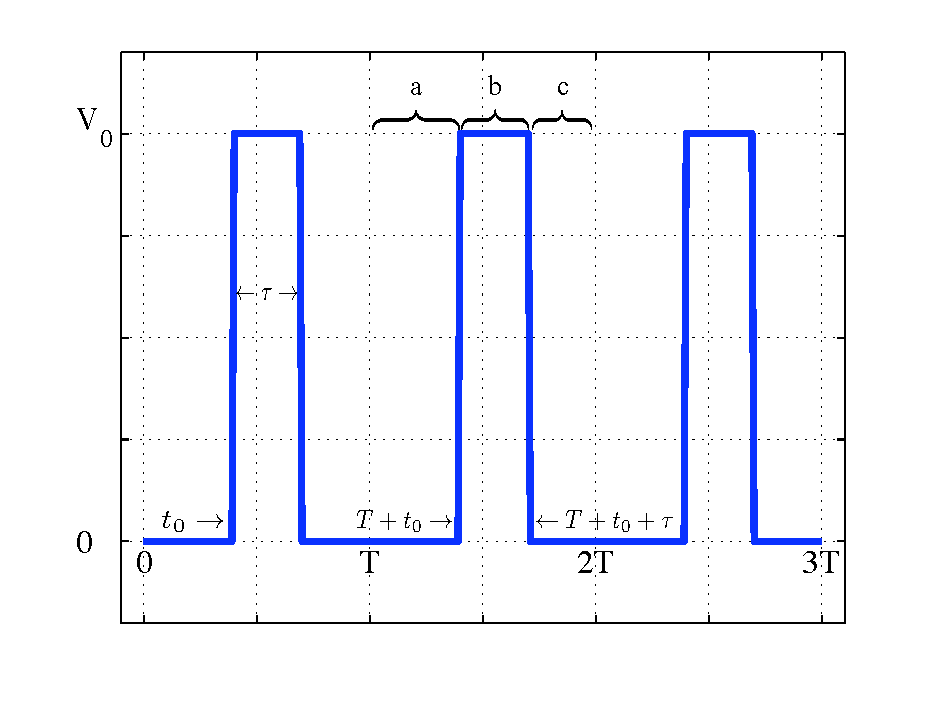
\includegraphics[width=5in]{ch-physical/fs_pulse}}
\caption[A train of periodic rectangular pulses]{A train of periodic
rectangular pulses with period $T$, pulse width $\tau$, and
initial pulse start at $t_0$.
\label{fig:fs-pulse}}
\end{figure}

There are a few general observations we can make of this signal: the
first, that the pulse duration $\tau$ is a variable, so it can be wide
or narrow, thus changing the duty cycle. When it is really narrow, the
signal becomes a train of impulses; when it is on the order of
$\tau=T/2$, it is called ``50\% duty cycle''. The second observation
is that $t_0$ changes the pulse's phase.

According to~(\ref{eq:fs-ck}), the Fourier coefficients $c_k$ are
\begin{align}
c_k &= \frac{1}{T}\int_0^{t_0} 0e^{-jk\omega_0 t} dt
      +\frac{1}{T}\int_{t_0}^{t_0+\tau}V_0e^{-jk\omega_0 t}dt 
      +\frac{1}{T}\int_{t_0+\tau}^{T}0e^{-jk\omega_0 t}dt 
      \label{eq:sq-fs1}\\
    &=\frac{1}{T}\int_{t_0}^{t_0+\tau}V_0e^{-jk\omega_0 t}dt 
      \label{eq:sq-fs2}\\
    &=\frac{V_0}{T}\left[\frac{e^{-jk\omega_0t}}
                               {-jk\omega_0}\right]_{t_0}^{t_0+\tau}
       \label{eq:sq-fs3}\\
    &=\frac{V_0}{-jk\omega_0T}[e^{-jk\omega_0(t_0+\tau)}
                               -e^{-jk\omega_0(t_0)}]
\label{eq:fs-pul-cn1}
\end{align}
In equation~(\ref{eq:sq-fs1}), the integral defining the Fourier
coefficients in~(\ref{eq:fs-ck}) has been broken into three parts for
the three ``segments'' of the square wave: $f(t)=0$ (region a, when $nT\leq t <
nT+t_0$), $f(t)=V_0$ (region b, when $nT+t_0 \leq t < nT+t_0+\tau$), and
$f(t)=0$ (region c, when $nT+t_0+\tau \leq t < (n+1)T$). The first and third
terms are equal to zero, leaving only the middle term, which is just
the integral of an exponential. If we remember that the derivative of
an exponential $\deriv{e^{at}}{t}$ is $ae^{at}$, then the
anti-derivative from~(\ref{eq:sq-fs2}) to~(\ref{eq:sq-fs3}) should
make sense. Finally, we just need to evaluate the expression
in~(\ref{eq:sq-fs3}) between the two limits $t_0$ and $t_0+\tau$ to
yield~(\ref{eq:fs-pul-cn1}).

The middle steps are left for your homework; let's skip to the result:
\begin{equation}
c_k=
  \underbrace{\frac{V_0\tau}{T}
     \frac{\sin(k\omega_0\tau/2)}{k\omega_0\tau/2}}_{\mathrm{magnitude}}
  \underbrace{e^{-jk\omega_0(t_0+\tau/2)}}_{\mathrm{phase}}
\label{eq:fs-pul-cn2}
\end{equation}
This is just the polar representation of a complex valued $c_k = R
e^{j\theta}$.  The phase $\theta$ or angle of $c_k$ is
\begin{equation}
\theta=-k\omega_0 \left(t_0+\frac{\tau}{2}\right)
\end{equation}
Let's define $\alpha=k\omega_0 \tau/2$, and take a look at the
magnitude in~(\ref{eq:fs-pul-cn2}). This function occurs frequently
enough in modern communication theory to be given a name: the sampling
function, or \emph{sinc}. We define
\index{sinc function}

\begin{equation}
\sinc\alpha = \frac{\sin\alpha}{\alpha}
\end{equation}

We note that $\sinc\alpha$ is zero whenever $\alpha$ is an integral
multiple of $\pi$; that is,
\begin{equation}
\sinc n\pi = 0, \quad n=1, 2, 3, \ldots
\label{eq:fs-Snpi}
\end{equation}

When $\alpha$ is zero, the function is indeterminate, but it is easy
to show that its value is unity: 
\begin{equation}
\sinc 0 = 1
\label{eq:fs-S0}
\end{equation}

\begin{figure}
\centerline{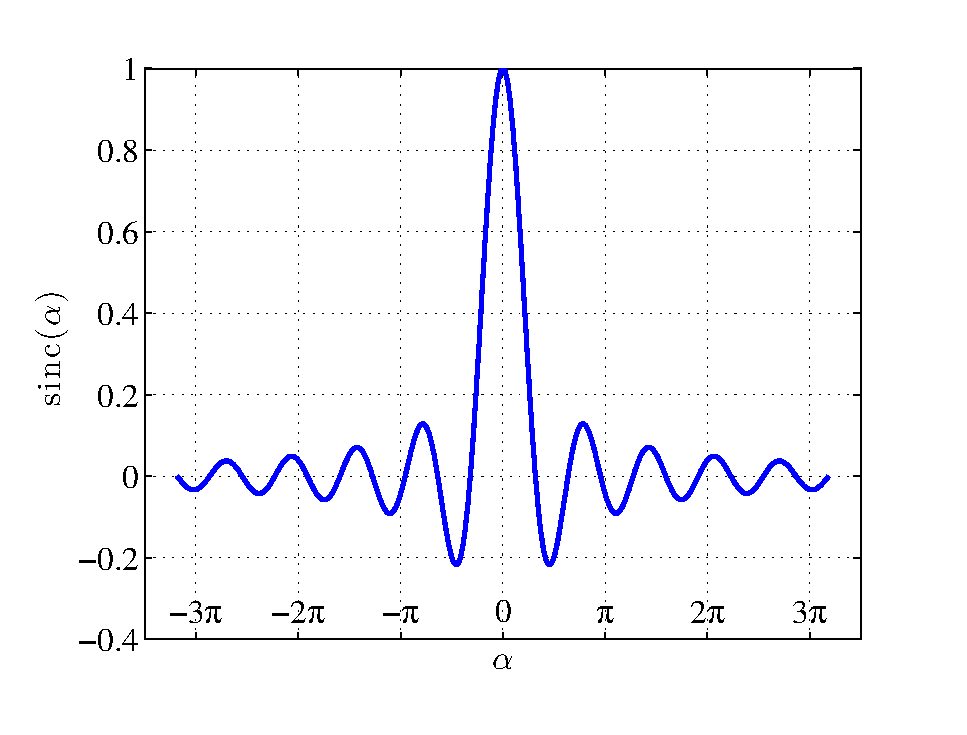
\includegraphics[height=3in]{ch-physical/fs_sinc}}
\caption{The sinc function.\label{fig:sinc}}
\end{figure}

The magnitude of $\sinc\alpha$ therefore decreases from unity at
$\alpha=0$ to zero at $\alpha=\pi$. As $\alpha$ increases from $\pi$
to $2\pi$, $\sinc\alpha$ increases from zero to a maximum less than
unity. As $\alpha$ continues to increase, the successive maxima become
smaller because the numerator of $\sinc\alpha$ can not exceed unity
while the denominator increases. Also, $\sinc\alpha$ shows even
symmetry. Figure~\ref{fig:sinc} shows the sinc function.

From~(\ref{eq:fs-S0}), we know that $c_0$ is 
\begin{equation}
c_0=\frac{V_0\tau}{T}
\end{equation}

Substituting $c_0$ and $c_k, k=1, 2,3,\ldots$
into~(\ref{eq:fs-freal1}), the Fourier series of $f(t)$ is
\begin{align}
f(t)&= \frac{V_0\tau}{T} +2\Real\left\{\sum_{k=1}^{\infty}
          \frac{V_0\tau}{T}
          \frac{\sin(k\omega_0\tau/2)}{k\omega_0\tau/2}
          e^{-jk\omega_0(t_0+\tau/2)}e^{jk\omega_0t}\right\} 
       \label{eq:fs-pulsef1}\\ 
    &= \frac{V_0\tau}{T}
       + 2\Real\left\{\sum_{k=1}^{\infty}\frac{V_0\tau}{T}
            \frac{\sin(k\omega_0\tau/2)}{k\omega_0\tau/2}
            e^{jk\omega_0(t-t_0-\tau/2)}\right\} && \text{(collect exponents)}
       \label{eq:fs-pulsef2}\\
    &= \underbrace{\frac{V_0\tau}{T}}_{c_0}
       + \underbrace{\frac{2V_0\tau}{T} \sum_{k=1}^{\infty}
           \sinc(k\omega_0\tau/2)}_{c_k}
           \underbrace{\cos[k\omega_0(t-t_0-\tau/2)]}_{\text{harmonically
               related sinusoids}} && \text{(apply Euler's)}
\label{eq:fs-pulsef}
\end{align}
In~(\ref{eq:fs-pulsef1}), we have used the knowledge of this being a
real-valued signal. We collected the exponents to
get~(\ref{eq:fs-pulsef2}), then factored out the $V_0\tau/T$, applied
Euler's formula to the exponential, and finally retained only the real
part of each term of the summation to yield~(\ref{eq:fs-pulsef}).

\begin{figure}
\centerline{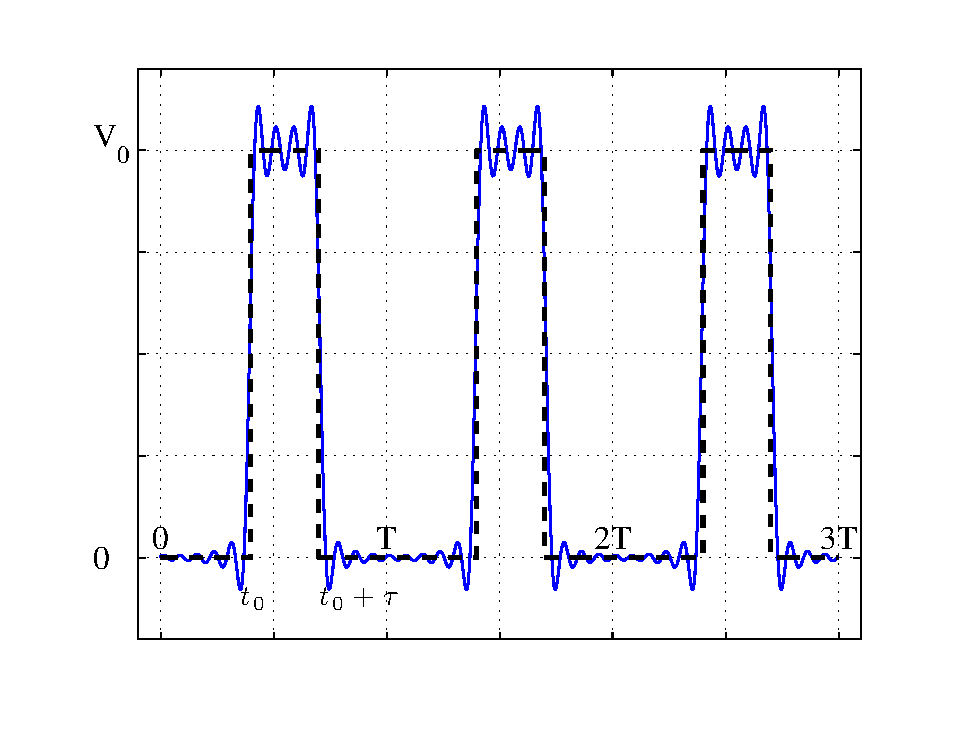
\includegraphics[width=5in]{ch-physical/fs_pulsef12}}
\caption[First 12 terms in the Fourier series for a periodic sequence
of rectangular pulses]{The Fourier series for a periodic sequence of
rectangular pulses. The first 12 harmonic terms in
summation~(\protect\ref{eq:fs-pulsef}) are included. The ideal pulse
train is shown as dashed lines. The period is $T=1$, the initial point
$t_0=0.5$ and the pulse width $\tau=0.3333$.
\label{fig:fs-pulsef}}
\end{figure}

\begin{figure}
\centerline{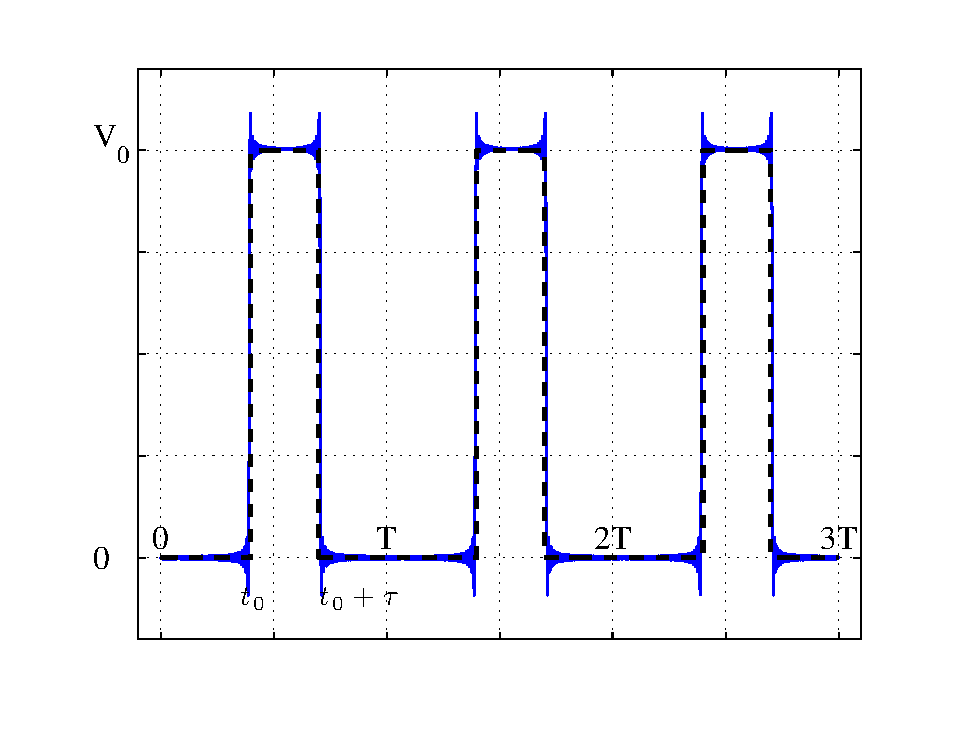
\includegraphics[width=5in]{ch-physical/fs_pulsef100}}
\caption[First 100 terms in the Fourier series for a periodic sequence
of rectangular pulses]{The Fourier series for a periodic sequence of
rectangular pulses. The sum of the first 100 terms is shown, as in
figure~\protect\ref{fig:fs-pulsef}.
\label{fig:fs-pulsef2}}
\end{figure}

Now, a train of pulses is represented by an infinite number of
sinusoidal waves. How well can it be approximated by a finite number?
Look at figure~\ref{fig:fs-pulsef}. The solid curve shows the sum of
the first 12 terms of the signal's Fourier series; it looks like a
pulse train modulated by a sinusoid. The ideal pulses are shown as
dashed lines. The approximation gets better when more terms are used,
as in figure~\ref{fig:fs-pulsef2}.

Let's construct the signal's \emph{spectrum}: a plot of its Fourier
\index{spectrum}
coefficients. We first consider $|c_k|$ expressed in terms of the
fundamental frequency $f_0$, remembering that $\omega_0=2\pi f_0$:
\begin{equation}
|c_k|=\frac{V_0\tau}{T}|\sinc(k\pi f_0 \tau)|
\label{eq:fs-pulseabscn}
\end{equation} 

The magnitude of any $c_k$ is obtained from~(\ref{eq:fs-pulseabscn})
by using the known values of pulse width $\tau$ and signal period
$T=1/f_0$, and selecting the desired value of $k$ $(k=0, 1, 2,
\ldots$). Instead of evaluating~(\ref{eq:fs-pulseabscn}) at these
discrete frequencies, let us sketch the envelope of $|c_k|$ by
considering the frequency $kf_0$ to be a continuous variable. That is,
though $f=kf_0$ can really only take on the discrete values (the
harmonic frequencies - $0, f_0, 2f_0, 3f_0, \ldots$) we may think
of $k$ for the moment as a continuous variable. When $f$ is zero,
$|c_k|$ is $V_0\tau/T$, and when $f$ has increased to
$1/\tau$, $|c_k|$ is zero.  In fact from (\ref{eq:fs-Snpi}) when
$f\pi\tau = m\pi$ ($m=1,2,3,\ldots$), $\sinc(f\pi\tau)=0$, which
yields zeros at frequencies $f = m/\tau$.

\begin{figure}
\centerline{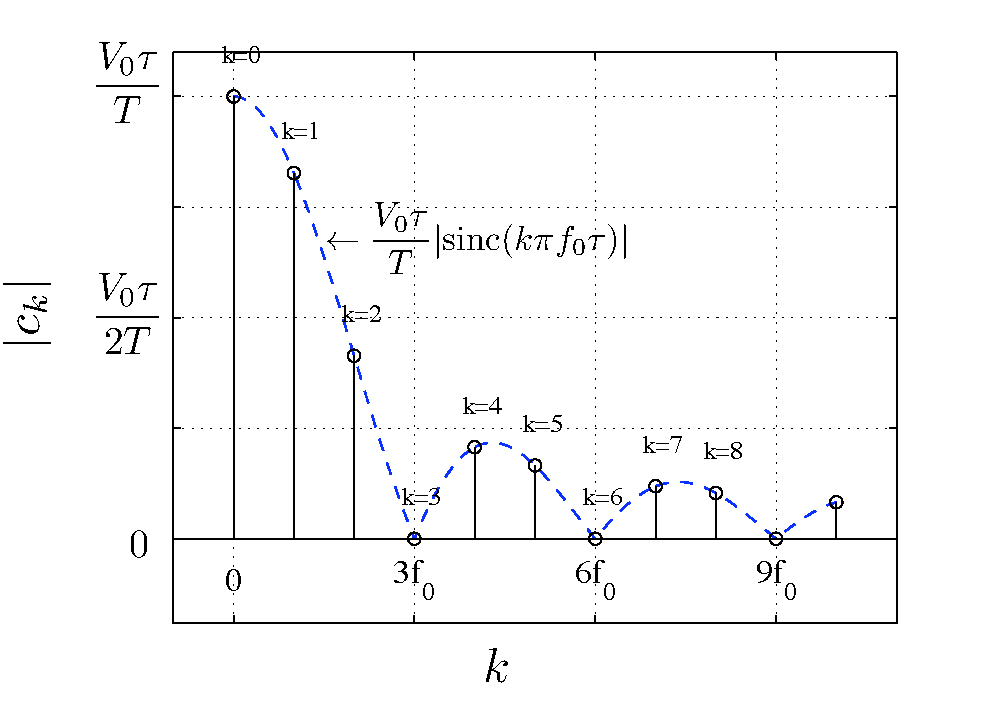
\includegraphics[height=4in]{ch-physical/fs_pulsecn}}
\caption[Spectrum of a periodic sequence of rectangular pulses]{The
spectrum of a periodic sequence of rectangular pulses: the magnitude
of $c_k$ vs. frequency $f=kf_0$, where $f_0=1/T$ (light gray vertical
lines).  The envelope for continuous $k$ is plotted as the black
curve. Zero points in the spectrum $|c_k|$ are at $kf_0=n/T=m/\tau$,
$m=1,2,3,\ldots$.
\label{fig:fs-pulsecn}}
\end{figure}

The resultant line spectrum and envelope are plotted in
figure~\ref{fig:fs-pulsecn}.  The figure is the plot of the envelope
of the Fourier coefficients $\{c_k\}$ (the spectrum of the periodic
sequence of rectangular pulses), versus frequency $f=kf_0$. The
magnitude of its peaks decays at the rate of $1/k$.

\begin{figure}
\centerline{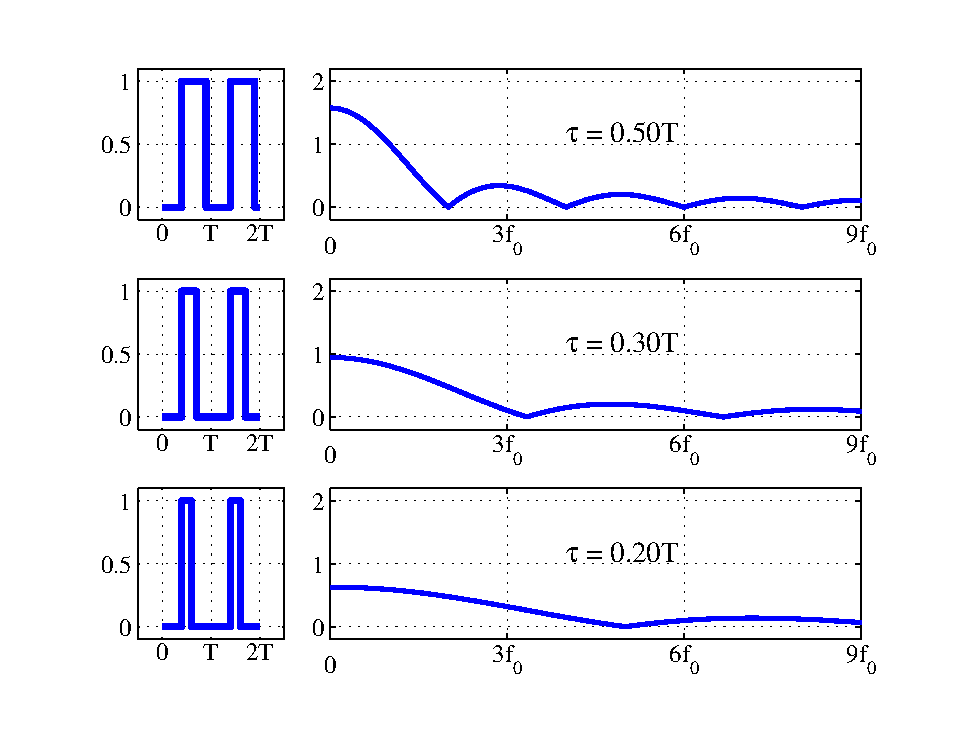
\includegraphics[height=4in]{ch-physical/fs_pulsecntau}}
\caption[Spectrum of a periodic sequence of rectangular 
pulses; varying pulse width]{The spectrum of a periodic sequence of
rectangular pulses, when $T$ is fixed and the pulse width $tau$
varies.
\label{fig:fs-pulsecntau}}
\end{figure}

\begin{figure}
\centerline{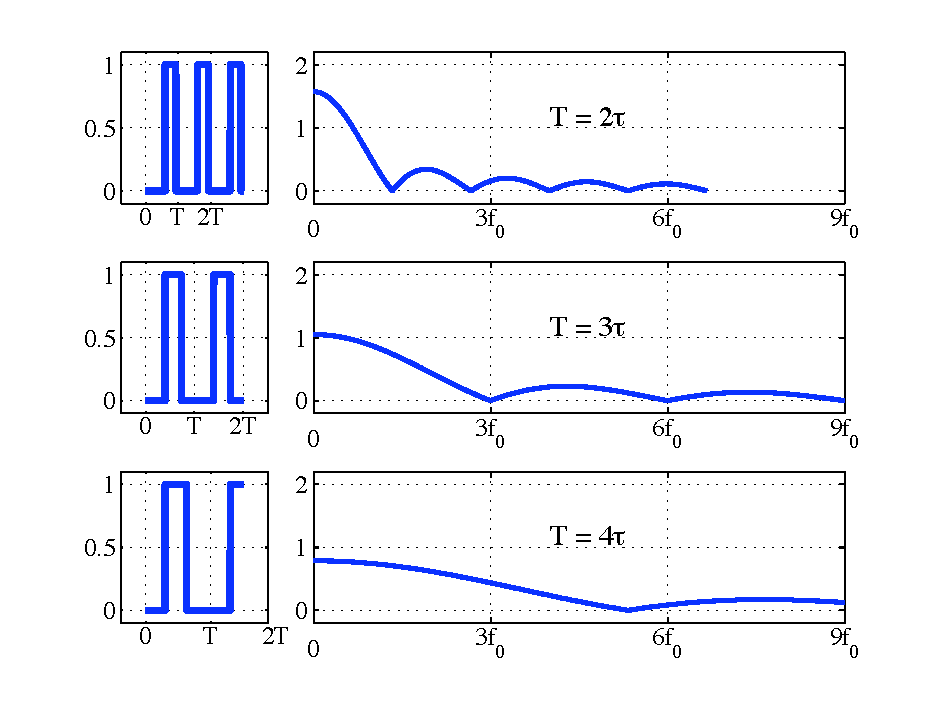
\includegraphics[height=4in]{ch-physical/fs_pulsecnT}}
\caption[Spectrum of a periodic sequence of rectangular  
pulses; varying period]{The spectrum of a periodic sequence of
rectangular pulses with fixed pulse width $tau$ and varying period
$T$.
\label{fig:fs-pulsecnT}}
\end{figure}

There are several observations which we may make that relate
changes in the line spectrum to changes in the graph of rectangular pulses
given in figure~\ref{fig:fs-pulsecn}. Firstly, note that the width of the envelope
depends upon changes in $\tau$, the pulse width. In fact,
the \emph{shape} of the envelope does not vary with changes in $T$;
instead, changes in $T$ correspond to changes in the frequency
interval between spectral lines. If the pulse period $T$ is increased
($f_0$ is decreased), the number of spectral lines between zero
frequency and $1/\tau$ increases and the amplitude of each line
decreases. Figures~\ref{fig:fs-pulsecntau} and~\ref{fig:fs-pulsecnT}
illustrate this.

A shift in the phase $t_0$ does not change the line spectrum,
that is, $|c_k|$ is not a function of $t0$. The \emph{phase} of the
frequency components \emph{do} change with the choice of $t_0$ (we just
haven't plotted those).

When talking about the generalized square wave, with fixed period $T$
and pulse width $\tau$ increasing or decreasing, the result is a
family of different waveforms. When $\tau = T/2$, we have a 50\% duty
cycle square wave. When $\tau$ takes on different percentages of $T$,
we get different duty cycles. Also, when $\tau$ becomes really small,
the waveform become a train of impulses.

\problemset{
\subsubsection{Self-Test Exercise}

See~\ref{sc:ch1ex} \#\ref{it:ch1ex10} for the answer.

\begin{enumerate}
\item Prove (\ref{eq:fs-S0}).
\end{enumerate}}



\section{Problems}

\begin{enumerate}
\item The differential equation for a tuning fork can be written as $\sderiv{x(t)}{t} = -\frac{k}{M} x(t) $ where $M$ is the mass of the tuning fork, $k$ is a constant, and $x(t)$ is the displacement of the tuning fork endpoints. Discuss how the mass of the tuning fork affects the frequency at which it vibrates. Hint: relate the given equation to equation \ref{eq:diffeq1}.
\item What musical instruments might be governed by properties
  analogous to that of a tuning fork? 
\item When you add two sinusoids with frequencies that differ by
  $\delta$, the result is beating. Imagine you're tuning a guitar.  As
  the two strings get closer together in tone, what happens to the
  beat frequency? Show how this result is predicted by the sum of the
  complex sinusoids.
\item A complex number can be written in rectangular coordinates as $z
  = x + j y$. Write the relations to calculate the polar form, $z=(r,
  \theta)$ or $z = r e^{j\theta}$.

\item Using Euler's formula, express $\cos x$ and $\sin x$ as a
  combination of complex exponentials. Recall that Euler's Formula is given by: $e^{\pm j\omega t}=\cos(\omega t) \pm j \sin(\omega t)$.

\item Find expressions for the following as complex exponentials:
	\begin{enumerate}
	\item1 
	\item $j$
	\item $1 + j$, $(1 + j\sqrt{3})/2$
	\end{enumerate}

\item Compute $[(1+j\sqrt{3})/2]^2$ and $(1+j)^4$ directly using: 
  \begin{enumerate}
  \item Rectangular representations.
  \item Complex exponentials.
  \end{enumerate}

\item Show that $(z_xz_y)^* = z_x^* z_y^*$.


\item Express $|z|^2$ as a function of $z$ and $z^*$.


\item Given the following equations:
\begin{align*}
x_1(t) &= 5 \sin(2\pi(200)t +0.5\pi) \\
x_2(t) &= 5 \sin(2\pi(200)t - 0.25\pi) \\
x_3(t) &= 5 \sin(2\pi(200)t +0.4\pi) \\
x_4(t) &= 5 \sin(2\pi(200)t - 0.9\pi) 
\end{align*}

\begin{enumerate}
\item Using pencil and paper: Express   $x_1(t)$ through $x_4(t)$ as complex exponentials. 

\item Create the sum sinusoid, $x_5(t)=x_1(t)+x_2(t)+x_3(t)+x_4(t)$. Express   $x_5(t)$ as a sum of complex exponentials. 	

 \item Using complex exponentials, express the amplitude and phase of $x_5(t)$ (use pencil and paper with the aide of a graphing calculator, spreadsheet, or MATLAB).

 \end{enumerate}
	
\item What is the period of $e^{-j\frac{\pi}{4}t}+e^{-j\frac{\pi}{2}t}$ ?
\item What is the period of $e^{-j \omega_0 t}+e^{-j 5\omega_0 t}$ ?
\item Implement a  \texttt{Complex} class for representing
  complex numbers in an object oriented programming language (C++, C\#, Java, python, etc.).  Your class should include at least the following
  methods:
  \begin{itemize}
  \item \texttt{add()}
  \item \texttt{multiply()}
  \item \texttt{real()}
  \item \texttt{imag()}
  \item \texttt{magnitude()}
  \item \texttt{angle()}
  \end{itemize}

  Document your code so that this class could be used by someone else.
  Write a test program that exercises all of this class' methods. 

\item Derive equation~(\ref{eq:fs-pul-cn2}) from
  equation~(\ref{eq:fs-pul-cn1}).

\item Determine the coefficients of the Fourier series for the following signals:
\begin{enumerate}
\item The sinusoid \[x(t) = \cos \frac{\pi}{3} t\]
\item The sawtooth waveform \[ x(t) = t-\lfloor t \rfloor \]
\item The rectified wave \[ x(t) = |\cos(\frac{\pi}{3} t)| \]
\end{enumerate}
\end{enumerate}

\section{Further Reading}

\begin{itemize}
\item James H McClellan, Ronald W. Schafer, and Mark A. Yoder,
  \textit{DSP First: A Multimedia Approach}, Prentice Hall, 1998,
  chapters 1--3 (\S 3.1--3.4), appendix A.
\item Martin D. Levine, \textit{Vision in Man and Machine},
  McGraw-Hill, 1985, chapter 1, sections 2.1, 2.2.
\item Robert S. Tannenbaum, \textit{Theoretical Foundations of
  Multimedia}, Computer Science Press, 1998, chapters 1 \& 2.
\item Donald Hearn \& M. Pauline Baker, \textit{Computer Graphics},
  Second Edition, Prentice Hall, 1997, sections 2.1--2.4.
\item A. Murat Tekalp, \textit{Digital Video Processing}, Prentice
  Hall, 1995, chapters 1 \& 2. 
\end{itemize}

